% ============================================================================
% Applied Sciences (MDPI) 投稿主文件
% 模板：官方 MDPI_template_ACS（mdpi.cls，更新于 2026-09-11），严格未改
% 作者：黄金辉（单一作者，oneauthor）
% 纪律：
%   1. 本文件为**纯手工书写的 LaTeX 源码**，任何自动化脚本不得对正文做
%      转义处理（上一轮投稿曾因 \footnotesize 的 "\f" 被脚本当转义字符吞掉，
%      导致 PDF 中出现 "ootnotesize" 文本压在表题上，构成"图文重叠"事故）。
%   2. 所有数字必须与 logs/*.json 及《项目事实台账》一致。
%   3. 图片文件名与 figures/ 目录一致，缺图不得进入编译。
% ============================================================================
\documentclass[journal,article,submit,oneauthor]{Definitions/mdpi}

%--------------------------------------------------------------------
% 数学宏包（mdpi.cls 未内置，按模板说明在导言区允许自行添加）
%--------------------------------------------------------------------
\usepackage{algorithm}
\usepackage{algpseudocode}
\makeatletter
% mdpi.cls 已加载 amsmath；algorithmic 的命名与 mdpi 的数学环境不冲突
\makeatother

%--------------------------------------------------------------------
% MDPI internal commands (do not modify)
%--------------------------------------------------------------------
\firstpage{1}
\makeatletter
\setcounter{page}{\@firstpage}
\makeatother
\pubvolume{1}
\issuenum{1}
\articlenumber{0}
\pubyear{2026}
\copyrightyear{2026}
\datereceived{}
\daterevised{}
\dateaccepted{}
\datepublished{}

%--------------------------------------------------------------------
% 初稿清理（作者指示 2026-10-13）：以下"录用后"装饰元素在初稿中隐藏——
%   ① 左栏空日期（Received/Accepted/Published）与 Copyright/CC-BY 块；
%   ② 页眉 "Version ... submitted to Journal Not Specified"；
%   ③ 页脚 "https://doi.org/..."（占位 DOI）；
%   ④ 首页右上角 MDPI 徽标。
% 实现方式：仅在导言区覆盖类命令（\patchcmd / \fancypagestyle），不改模板本体；
% 页眉右上角页码 "N of M" 保留，供审稿定位。
%--------------------------------------------------------------------
\makeatletter
\renewcommand{\leftcolDates}{}%
\renewcommand{\leftcolumnCright}{}%
\makeatother

\makeatletter
\AtBeginDocument{%
  % 页眉页脚：全部页只保留右上角 "N of M"
  \fancypagestyle{plain}{%
    \fancyhf{}%
    \fancyhead[R]{\fontsize{8}{8}\selectfont\thepage{} of \pageref*{LastPage}}%
    \renewcommand{\headrulewidth}{0pt}%
    \renewcommand{\footrulewidth}{0pt}%
  }%
  \fancyhf{}%
  \fancyhead[R]{\fontsize{8}{8}\selectfont\thepage{} of \pageref*{LastPage}}%
  \renewcommand{\headrulewidth}{0pt}%
  \renewcommand{\footrulewidth}{0pt}%
  % 首页右上角 MDPI 徽标：从 \@maketitle 的 submit 分支中移除
  \patchcmd{\@maketitle}%
    {\hfill \href{https://www.mdpi.com}{
\includegraphics[height=1cm]{Definitions/logo-mdpi.eps}}}%
    {\hfill}%
    {}{\PackageWarning{cleandraft}{MDPI logo patch failed}}%
}
\makeatother

%--------------------------------------------------------------------
% Title / Authors
%--------------------------------------------------------------------
\Title{Auditable Anomaly Detection for Unattended Delivery Lockers:
A Calibrated Rule Pipeline with Field-Footage Boundaries and a Pre-Deployment Audit}

\newcommand{\orcidauthorA}{0009-0004-3070-5092}

\Author{Jinhui Huang $^{1,}$*\orcidA{}}

\AuthorNames{Jinhui Huang}

\address{%
$^{1}$ \quad College of Computer and Artificial Intelligence, Northeast Forestry University,
Harbin 150040, China; 2088239568@qq.com}

\corres{Correspondence: 2088239568@qq.com}

%--------------------------------------------------------------------
% Applied Sciences featured application (optional, encouraged)
%--------------------------------------------------------------------
\featuredapplication{The calibrated, rule-based pipeline described in this paper provides an
auditable and CPU-only monitoring layer for unattended delivery lockers and other
grid-structured self-service cabinets. A two-part pre-deployment audit---a geometric check
and a colour-domain collision check---predicts, before alarms are enabled, whether a given
site needs recalibration or colour-model adjustment.}

%--------------------------------------------------------------------
% Abstract
%--------------------------------------------------------------------
\abstract{Unattended delivery lockers are now public infrastructure, yet their operation
is supervised only passively: cameras, when present, serve forensics rather than
proactive alerting. This paper develops and evaluates an auditable anomaly
detection layer for a campus food-delivery locker under a deliberately constrained
budget---one CPU-only computer, open-source components, fully local processing.
The system estimates each compartment's open/closed state from calibrated regions, tracks users, and raises six event types through per-compartment rules
whose thresholds are all named parameters, so every alarm can be audited: it names a compartment, a measured quantity and a threshold. Evaluation proceeds in
three tiers. On a 119-clip rendered benchmark the pipeline attains perfect clip- and
event-level scores, read as implementation verification, not a generalization
estimate; a paired ablation attributes the gain to
re-association, and an analytic replay bounds the door-alarm threshold without
re-runs. On 15 field recordings from six installations, uncalibrated
deployment emits one event every 4.4~s (197 of 261 are alarms), whereas a real
door-left-open episode is detected by the system's darkness-ratio statistic with a
wide margin (0.94 against a 0.15 threshold, controls below 0.04). Finally, a two-part
pre-deployment audit---geometric coverage and clothing-versus-package colour collision
(28.3\% of person-frames)---predicts which rules misfire at a new site.}

\keyword{anomaly detection; unattended delivery locker; edge vision; behaviour state machine;
auditable rule engine; CPU-only inference}

\begin{document}

%%%%%%%%%%%%%%%%%%%%%%%%%%%%%%%%%%%%%%%%%%
\section{Introduction}
\label{sec:intro}

Cities increasingly depend on \emph{unattended} service infrastructure: parcel lockers,
food-delivery cabinets, self-service kiosks and similar facilities that store, transfer and
release goods without a member of staff present. The scale of this layer is no longer
marginal. Parcel-locker networks are treated in logistics research as a fixed element of
last-mile planning~\cite{lai2021parcel,li2025parcel,zhang2025campus}, smart-retail studies
treat automated pickup points as a standard channel~\cite{pantano2014smart}, and the
facilities themselves are now part of campus, residential and transit environments. These
installations share three properties that make them an interesting computer-vision problem.
First, they hold third parties' property around the clock, so losses and contamination are
attributed through the facility rather than to a visible person. Second, they operate in
public space where the only pervasive sensor is a camera, and where privacy requirements
push processing towards the edge~\cite{shi2016edge,ribaric2016deid}. Third, and least
explored, their failures are \emph{operational} rather than dramatic: a compartment left
ajar, food collected by the wrong person, a package taken from a compartment somebody else
left open. Cameras at such sites, when they exist at all, are used forensically---footage is
reviewed after a complaint. The supervision gap is therefore not one of signal quality but
of \emph{timeliness and accountability}: nobody is alerted while the door stands open, and
when an alert does come, the operator must be able to answer which compartment, which
quantity, and which threshold produced it.

Figure~\ref{fig:context} shows examples of the installations this paper targets, drawn
from publicly available recordings of real locker use. This paper studies that gap on a concrete instance: a campus food-delivery locker served by
a single low-cost computer. The scenario was selected because it concentrates the general
problem in a measurable form. A project-team survey of campus users (120 valid responses out
of 130; described in Section~\ref{sec:setup}) found that 86.7\% of respondents consider
current locker use to carry security risks, 91.7\% support automated behaviour recognition,
88.3\% require the supervision to be non-intrusive, and 74.2\% are concerned about
low-illumination operation. From the operational vocabulary of the site---obtained by
mapping the survey's risk statements onto directly observable states---four alarm classes
emerge: a compartment door left open after a retrieval, one person collecting two or more
packages, a package collected from a compartment that a previous user left open, and
loitering without retrieval. Each corresponds to a state that a calibrated vision pipeline
can \emph{measure} rather than a behaviour that must be \emph{classified}: a timer on a
compartment, a count of carried objects, a flag with a lifetime, an accumulated presence
time.

Building such a layer under the actual deployment budget---one CPU-only machine, no
additional sensors, open-source components, local processing only---implies a different
design point from the mainstream of video anomaly detection. Modern VAD research is
dominated by learned normality models, from reconstruction and prediction
autoencoders~\cite{duong2023vad} to weakly supervised spatio-temporal
transformers~\cite{zhong2025interclip} and vision-language
models~\cite{xu2025plovad,barbosa2026survey,wu2026vad}. These methods are powerful, but
they answer a different question: they score how unusual a clip is, and their output is not
attributable to a compartment or a person. For a facility whose operator must act on
specific, enumerable incidents and justify each action to customers, the useful primitive is
not an anomaly score but an \emph{auditable event}: a named condition over measured
quantities, produced by a rule that can be inspected, configured and unit-tested. The
trade-off is explicit---rule-based analytics must anticipate the behaviour vocabulary, while
learned models might discover unanticipated anomalies---and for a managed site with a fixed
set of operational concerns, the anticipatable direction is the favourable one.
\citet{lim2014isurveillance} made the same argument for rule-driven surveillance event
detection a decade ago; what has changed since is that the perception components (person
detectors, trackers) are now strong enough on commodity hardware that the remaining
difficulty is \emph{calibration and accountability}, not detection per se.

\begin{figure}[H]
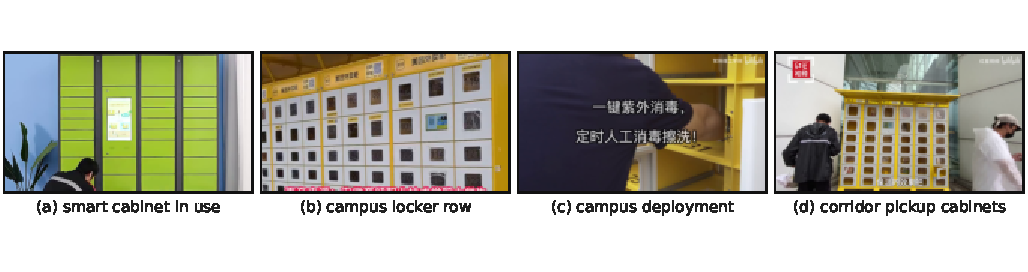
\includegraphics[width=0.98\textwidth]{figures/fig1_context.pdf}
\caption{The deployment domain, as it exists in the field: frames from publicly available
recordings of real locker use (Section~\ref{sec:field-corpus}). Left to right: a
manufacturer-branded smart cabinet in use; a campus food-locker row; a campus deployment
under installation; and a corridor of pickup cabinets during a contactless-delivery
trial. The installations differ in brand, cabinet
geometry, colour scheme, camera pose and illumination---the diversity that the calibration
and audit procedures of this paper are designed to handle. Frames are reproduced from
publicly available recordings; their published titles are listed in the Data Availability
Statement, and no recording is redistributed.\label{fig:context}}
\end{figure}

The design in this paper therefore treats the fixed deployment geometry as an asset: a
one-time calibration marks the pickup area and the compartment grid, and every subsequent
judgment---zone membership, door-state regions, proximity to a compartment---is expressed in
calibrated coordinates as pure functions. On top of this calibration sit three layers: a
detection-and-tracking stage with explicit guards against the failure modes we measured
(partial boxes, multi-second detector gaps, occlusion); a per-compartment door-state
estimator that decides open/closed from a contrast statistic relative to the frame's median
brightness, with person-pixels masked out and a hold policy for occluded states; and a rule
engine whose per-track and per-compartment state machines emit the six event types. Every
threshold is a named configuration parameter with a documented default, and several defaults
are non-arbitrary: they were widened or narrowed in response to measured failure modes, a
fact we document so that the configuration can be reproduced rather than guessed.

Evaluation is organized around what each class of evidence can support; the classes are
kept separate throughout. A 119-clip rendered behaviour benchmark, generated by the same scene
geometry as the calibration, establishes \emph{correctness under same-distribution
conditions}---it verifies that the implementation executes the specified decision procedure,
and we do not read it as an estimate of generalization. A paired ablation isolates the
contribution of each failure-repair mechanism, and an analytic replay over recorded event
timelines bounds the sensitivity of the main alarm threshold without re-running any video.
Beyond these controlled experiments, the paper adds two elements that speak directly to
deployment. First, a \emph{field-footage boundary study}: 15 recordings from six real locker
installations (roughly 20~min, multiple brands and cabinet layouts) are run through the
complete pipeline in both constrained and calibrated configurations; among these recordings
is a real, unambiguous door-left-open episode whose duration we measure, and against which
the system's own door statistic is validated (a calm 0.94 reading during the episode versus
a 0.15 threshold, with three neighbouring control compartments staying below 0.04). Second,
a \emph{pre-deployment audit procedure}: because the package detector is a colour-domain
proxy, saturated warm-toned clothing can be mistaken for carried packages---an effect we
observed on field footage and then quantified---so we define and validate a two-part audit
(geometric coverage plus clothing-versus-package colour collision) that predicts, before
alarms are enabled, which sites will produce spurious alerts under the default configuration.
On the field corpus, 28.3\% of person-frames carry collision risk (289 of 1020; Wilson
95\% CI 25.7--31.2\%), with a per-site spread from 6.9\% to 66.7\% that matches the observed
spurious-alarm pattern.

The contributions of this paper are:

\begin{itemize}
\item \textbf{An auditable problem formulation and system} (\S\ref{sec:problem}--\S\ref{sec:method}):
compartment-attributed anomaly detection for an unattended locker, in which every alarm
reduces to a named observable, a declared threshold and a measured value, so that an operator
can answer ``which door, which quantity, which threshold'' for any event.
\item \textbf{A formalized calibrated pipeline} (\S\ref{sec:method}): one-time calibration of
the compartment grid and pickup area; a statistical model of the door-state decision with
occlusion handling; a two-stage association scheme with geometric guards whose thresholds are
derived from measured detector behaviour; and event state machines whose alarm latency is
predictable from their parameters. An \emph{analytic replay} method for threshold sensitivity
is derived and self-verified against measured counts.
\item \textbf{A field-footage boundary study} (\S\ref{sec:field}): the behaviour of the
complete pipeline on 15 recordings from real installations, including the quantified failure
of uncalibrated transfer (approximately one spurious alarm per 4.4~s of footage), the
validation of the door statistic on a real open-door episode, and a taxonomy of the
deployment domain (brands, cabinet geometry, camera pose, illumination) that the corpus
covers.
\item \textbf{A pre-deployment audit procedure} (\S\ref{sec:field}): a geometric audit and a
colour-collision audit that convert the field findings into an installation-time checklist;
the collision measure is defined, measured across the corpus, and checked against the
observed spurious-alarm pattern.
\item \textbf{Reproducibility under a CPU-only budget} (\S\ref{sec:experiments}): a complete
open-source stack with measured per-stage costs, a HOG fallback, and a demonstration that the
full pipeline sustains real-time operation on a single commodity computer, together with the
measured envelope---including per-frame cost decomposition and the multi-view scaling
limit---at which this claim holds.
\end{itemize}

The remainder of this paper is organized as follows. Section~\ref{sec:related} reviews
related work. Section~\ref{sec:problem} formulates the problem and describes the system
design; Section~\ref{sec:method} details the methods and their parameterization.
Section~\ref{sec:setup} describes the experimental setup, including the field corpus;
Section~\ref{sec:experiments} reports the controlled experiments; Section~\ref{sec:field}
reports the field-footage boundary study and the audit validation.
Section~\ref{sec:discussion} discusses boundaries and implications, and
Section~\ref{sec:conclusions} concludes.

%%%%%%%%%%%%%%%%%%%%%%%%%%%%%%%%%%%%%%%%%%
\section{Related Work}
\label{sec:related}

\subsection{Unattended facilities and locker supervision}
The literature on delivery lockers is dominated by logistics questions---location planning,
utilization, customer satisfaction---rather than by supervision. Parcel-locker network design
has been studied with p-median formulations on real trip data~\cite{li2025parcel}, and
user-centric locker selection has been optimized for campus last-mile
logistics~\cite{zhang2025campus}; both lines of work treat the locker as an interface for
handover, not as a monitored space. Camera-based supervision of such facilities is scarce.
The closest works detect the open/closed state of a door or the presence of objects inside a
single controlled cabinet, typically with a frontal calibrated camera and a single
per-cabinet decision~\cite{ramoa2021door}; retail-vision surveys reach the analogous
conclusion for shelf and cabinet item recognition~\cite{santra2019retail}. Two requirements
distinguish the present setting: an alarm must name one compartment among many, and it must
be attributable to a tracked person. Both are absent from cabinet-level methods, which
aggregate visual evidence into one decision before any identity is established. The system
studied here instead treats each compartment as an independently monitored entity, which is
precisely what makes per-compartment alarms---and their audit---possible.

\subsection{Video anomaly detection}
Video anomaly detection (VAD) has moved through reconstruction- and prediction-based
autoencoders, one-class and density models, weakly supervised multiple-instance learning over
spatio-temporal backbones, and---most recently---multimodal and vision-language
approaches. Recent surveys map this trajectory comprehensively~\cite{duong2023vad,
wu2026vad,barbosa2026survey}: Wu et al.~\cite{wu2026vad} organize the field from task
settings to foundation-model trends, and Barbosa et al.~\cite{barbosa2026survey} synthesize
multimodal and weakly supervised approaches; sequence-level methods continue to improve
fine-grained temporal localization~\cite{zhong2025interclip}, and open-vocabulary detection
is being re-purposed for VAD through promptable vision-language models~\cite{xu2025plovad}.
Edge deployment is an explicit concern of this literature: lightweight two-branch systems
target consumer hardware, and low-light smart-camera pipelines distribute enhancement and
detection across IoT-edge devices~\cite{abuawwad2024lowlight}. At the same time, a parallel
line argues for explicit knowledge in surveillance: rule-driven event detection frameworks
encode domain vocabulary directly~\cite{lim2014isurveillance}, loitering detection reduces to
a rule over tracked positions~\cite{zin2010loitering}, and recent hybrid systems blend
learned perception with rule-based or explanation mechanisms to make anomaly decisions
inspectable~\cite{fu2025iot,natha2025bilstm}. The position of the present work is close to
this last family, with one deliberate difference: not only the decision but also the
\emph{evidence chain} is rule-based. The system measures per-compartment states and tracked
positions, and every alarm carries the compartment number and the measured quantity that
crossed a threshold. This is what we call auditable anomaly detection, and it is the property
that makes the system usable for responsibility attribution in a shared facility---an
application requirement that generic anomaly scores do not satisfy, whatever their
accuracy~\cite{lim2014isurveillance}.

\subsection{Lightweight detection, tracking and edge deployment}
Efficient detectors from the YOLO family provide a practical accuracy--latency trade-off for
CPU deployment~\cite{redmon2016yolo,yolov8ultralytics}, and successive generations are
repeatedly benchmarked on embedded targets~\cite{reveles2025yolo11}; the smallest variants
are the standard choice when inference must share a machine with other
workloads~\cite{jia2025lpcf}. Classical descriptors such as HOG with a linear
SVM~\cite{dalal2005hog} remain relevant as degradation fallbacks rather than competitors.
Tracking-by-detection with data association supplies the identity that behaviour rules
require~\cite{zhang2022bytetrack}, and occlusion is the dominant failure mode of that
pipeline in surveillance settings; a recent survey systematizes occlusion handling across
the tracking
lifecycle~\cite{sun2025occlusion}. Two of the guards used in this paper---re-association
across multi-second detection gaps, and rejection of partial (upper-body) boxes---are
instances of the trajectory-recovery and track-management strategies catalogued there, with
thresholds derived from our own measurements rather than from generic defaults. Finally, the
edge-computing rationale---moving inference to the data for latency, cost and
privacy~\cite{shi2016edge}---is realized here in its strictest form: the entire pipeline,
including the operator console, runs on one machine and no video leaves it, with
de-identification-style privacy arguments~\cite{ribaric2016deid} satisfied by construction.
The measured cost decomposition and the multi-view scaling limit
(Section~\ref{sec:experiments}) are reported so that this claim is a quantity rather than a
slogan.
%%%%%%%%%%%%%%%%%%%%%%%%%%%%%%%%%%%%%%%%%%
\section{Problem Formulation and System Design}
\label{sec:problem}

\subsection{Scenario, geometry and notation}
\label{sec:notation}
A site consists of one locker bank and one fixed camera viewing it. The bank contains a known
set of compartments $\mathcal{K}=\{1,\dots,K\}$, physically arranged in rows and columns. The
camera is static during operation; its pose is arbitrary but chosen so that the compartment
fronts and the ground area in front of the bank are visible (the installation guidelines in
Section~\ref{sec:audit} state the practical conditions). Let $V$ denote the video, a sequence
of frames $v_t$ at source rate $f_s$; all processing is causal---decisions at time $t$ may
use frames up to $t$ only---and fully local.

Two coordinate systems are used. The \emph{image} system is the pixel grid of $v_t$, of size
$W\times H$. The \emph{panel} system is attached to the locker front, which is a plane
$\Pi$. For a point on $\Pi$ with panel coordinates $(X,Y)$, its image $\mathbf{x}=(x,y,1)$ is
given by the plane-induced homography
\begin{equation}
\label{eq:homography}
\mathbf{x} \;\sim\; \mathbf{H}\,\mathbf{X},
\qquad
\mathbf{H} \in \mathbb{R}^{3\times 3},
\qquad
\mathbf{X}=(X,Y,1)^{\top},
\end{equation}
where $\sim$ denotes equality up to scale. The homography is estimated once, during
installation, from correspondences between panel and image points (Section~\ref{sec:calib}),
and is fixed thereafter. Three derived structures are stored as \emph{normalized polygons}
(coordinates in $[0,1]^2$ relative to $W\times H$): the pickup-area polygon $P$, the
compartment polygons $\{C_k\}$, and---optionally---auxiliary zones. Storing polygons in
normalized coordinates makes every geometric query resolution-independent: for any frame
size, a polygon is mapped to pixels by scaling, and no threshold refers to absolute pixel
values. We return to the consequences of this invariance in Section~\ref{sec:exp-setup}.

A \emph{track} $\tau$ is a temporally coherent person hypothesis with a bounding box, a
stable identifier, a foot point $\phi(\tau)\in\mathbb{R}^2$ (bottom-centre of the box), a
last-seen timestamp $t_\tau$ and a trusted box height $\hat{h}_\tau$. A \emph{scene
observation} at time $t$ is the tuple
\begin{equation}
\label{eq:observation}
o_t \;=\; \bigl(\, \mathcal{D}_t,\; \{d_k(t)\}_{k\in\mathcal{K}},\;
\{n_k(t)\}_{k\in\mathcal{K}},\; \{c_\tau(t)\}_{\tau} \,\bigr),
\end{equation}
where $\mathcal{D}_t$ is the set of person detections, $d_k(t)\in\{\text{open},\text{closed},
\text{unknown}\}$ is the estimated door state of compartment $k$, $n_k(t)\in\mathbb{N}_0$ is
the number of package-like objects detected inside $C_k$, and $c_\tau(t)$ is the number of
package-like objects attributed to track $\tau$ as \emph{carried}. The rule engine consumes
the observation stream $\{o_t\}$ and emits events; its state is a finite set of per-track and
per-compartment variables.

\subsection{Event definitions}
\label{sec:events}
The system recognizes six event types (Table~\ref{tab:events}). Two are informational and
record the normal flow of a retrieval; four are alarms corresponding to the operational
concerns of Section~\ref{sec:intro}. Each alarm is defined as a predicate over the state
trajectories of the observation stream, not as a classification of a video segment. Writing
$T^{\mathrm{open}}_k(t)$ for the accumulated open time of compartment $k$ up to $t$ (defined
precisely in Section~\ref{sec:rules}), the four alarm predicates are:
\begin{align}
\textit{DoorLeftOpen}(k):&\quad
\exists t:\; T^{\mathrm{open}}_k(t)\ge \tau_{\mathrm{open}},
\label{eq:ev-door}\\[2pt]
\textit{MultiRetrieval}(\tau):&\quad
\exists t:\; c_\tau(t)\ge n_{\mathrm{multi}},
\label{eq:ev-multi}\\[2pt]
\textit{FlaggedRetrieval}(k):&\quad
\exists t:\; \bigl(f_k=1\bigr)\;\wedge\;\bigl(n_k(t^-)>n_k(t)\bigr),
\label{eq:ev-flag}\\[2pt]
\textit{Loitering}(\tau):&\quad
L_\tau(t)\ge \tau_{\mathrm{loit}}\;\wedge\; e_\tau\ge n_{\mathrm{entries}}
\;\wedge\; \mu_\tau<\tau_{\mathrm{peak}},
\label{eq:ev-loit}
\end{align}
where $\tau_{\mathrm{open}}=10$~s, $n_{\mathrm{multi}}=2$; $f_k$ is the flag set by
\eqref{eq:ev-door} and cleared when the compartment is confirmed closed
($\tau_{\mathrm{close}}=1.5$~s of consistent closed evidence); $L_\tau(t)$ is accumulated
nearby time, $e_\tau$ the entry count into the pickup area and $\mu_\tau$ the longest single
visit. The last conjunct of \eqref{eq:ev-loit} encodes a domain decision made with the site's
operators: a person who simply stands at the locker for a long single visit (waiting for a
phone lookup, reading messages) is \emph{normal}; loitering requires repeated approaches
without a long single visit. Events of the same type and the same target are suppressed
within a cooldown window $\tau_{\mathrm{cool}}=30$~s, and each suppression is counted in a
dedicated statistic so that the suppression rate is auditable rather than implicit.

\begin{table}[H]
\caption{The six event types, severities and default thresholds. Every threshold is a named
configuration parameter (Table~\ref{tab:params}); the cooldown between repeated events of
the same type and target is $\tau_{\mathrm{cool}}=30$~s.\label{tab:events}}
\small
\begin{tabularx}{\textwidth}{l l X}
\toprule
\textbf{Event} & \textbf{Severity} & \textbf{Trigger (default)} \\
\midrule
Pickup-area entry & info & foot point enters $P$ (debounced, 2 frames) \\
Door closed & info & flagged door confirmed closed for $\tau_{\mathrm{close}}=1.5$~s \\
Loitering & warning & nearby $\ge 15$~s with $\ge 3$ entries, no single visit $\ge 8$~s \\
Door left open & warning & compartment open $\ge \tau_{\mathrm{open}}=10$~s \\
Multiple packages & critical & one person carries $\ge n_{\mathrm{multi}}=2$ packages \\
Retrieval from flagged door & critical & package removed from a flagged compartment \\
\bottomrule
\end{tabularx}
\end{table}

Two properties of this vocabulary matter operationally. First, the alarms are
\emph{state-based}: each fires when a measured quantity crosses a declared threshold, which
is why the system raises them by rule rather than by classification, and why their firing
latency is predictable (Section~\ref{sec:replay}). Second, the vocabulary is
\emph{closed and configurable}: thresholds can be re-tuned per site without touching code,
and vocabulary items that other deployments might add (e.g., camera occlusion) are
deliberately absent because they are deployment conditions rather than user behaviours.

\subsection{Architecture and data flow}
\label{sec:arch}
Figure~\ref{fig:arch} summarizes the architecture; all stages run as threads of a single
process on one machine. A local video source feeds a detection--tracking stage that outputs
person boxes with stable identities. A scene-observation stage converts detections into the
structured observation of \eqref{eq:observation}: per-compartment visual evidence for the
door state, handheld package counts, and the zone of each tracked person. A rule engine then
evaluates the predicates of Section~\ref{sec:events} over the observation stream, maintains
per-track and per-compartment state, and emits events. Every event is persisted to a local
database together with a snapshot of its evidence frame; a web console---served from the same
machine, so that no video leaves the host---renders the live view with the calibrated grid
and per-compartment states overlaid, lists the event stream with thumbnails, and exposes the
configuration. The display loop and the detection loop are decoupled: display publishes the
newest frame to the detection thread, so a slow inference stage degrades the detection rate
but never the smoothness of the live view.

\begin{figure}[H]
%\isPreprints{\centering}{}
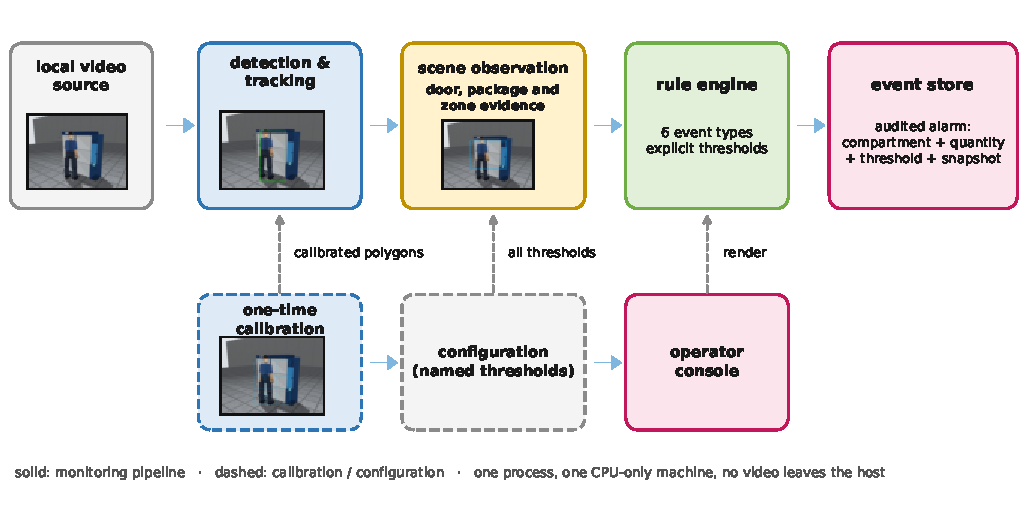
\includegraphics[width=0.98\textwidth]{figures/fig2_architecture.pdf}
\caption{System architecture. The solid path is the monitoring pipeline; every module runs
on a single CPU-only computer and no video leaves the machine. All thresholds live in one
configuration object; the calibration stage writes the geometric part of it. Events persist
with an evidence snapshot so that each alarm can be audited after the
fact.\label{fig:arch}}
\end{figure}

\subsection{Operating constraints}
\label{sec:constraints}
The design constraints, fixed before any method choice, are: (i) one personal computer with
CPU-only inference---no GPU, camera, or embedded accelerator; (ii) local video files or
image sequences as the only input source (no capture hardware); (iii) free and open-source
components only; and (iv) every threshold a named, documented configuration parameter rather
than a constant embedded in code. Constraints (i)--(iii) shape the perception stack
(lightweight detector, explicit fallback) and (iv) is what makes the pipeline auditable: an
administrator can inspect, justify and change every decision boundary, and the experiments
can vary thresholds analytically (Section~\ref{sec:replay}).

%%%%%%%%%%%%%%%%%%%%%%%%%%%%%%%%%%%%%%%%%%
\section{Method}
\label{sec:method}

\subsection{One-time calibration}
\label{sec:calib}
Because the deployment geometry is fixed and known, the system exploits it rather than
estimating it online. Calibration proceeds in two steps, supported by two interactive tools.
First, the pickup-area polygon $P$ is drawn once on a reference frame: it covers the ground
region in front of the bank where a retrieval user stands, and may exclude passage lanes. All
zone queries are point-in-polygon tests of the foot point $\phi(\tau)$ against $P$:
\begin{equation}
\label{eq:zone}
z(\tau) =
\begin{cases}
\text{pickup}, & \texttt{pointPolygonTest}(P,\phi(\tau)) \ge 0,\\
\varnothing, & \text{otherwise.}
\end{cases}
\end{equation}
Second, the compartment grid is fitted. The operator marks the four corners of the locker
panel (top-left, top-right, bottom-right, bottom-left) and declares the row and column
counts $(R,C)$; with a margin fraction $\mu$ that compensates for the frame width of each
door, the polygon of compartment $(r,c)$ ($0\le r<R$, $0\le c<C$) is generated by bilinear
interpolation of the panel corners $\mathbf{q}=(\mathbf{q}_{\mathrm{TL}},
\mathbf{q}_{\mathrm{TR}},\mathbf{q}_{\mathrm{BR}},\mathbf{q}_{\mathrm{BL}})$:
\begin{equation}
\label{eq:grid}
\mathbf{b}(u,v) \;=\; (1-v)\bigl[(1-u)\mathbf{q}_{\mathrm{TL}}+u\mathbf{q}_{\mathrm{TR}}\bigr]
\;+\; v\bigl[(1-u)\mathbf{q}_{\mathrm{BL}}+u\mathbf{q}_{\mathrm{BR}}\bigr],
\end{equation}
evaluated at the corners $\bigl(\frac{c+\mu}{C}, \frac{r+\mu}{R}\bigr)$, $\dots$,
$\bigl(\frac{c+1-\mu}{C}, \frac{r+1-\mu}{R}\bigr)$. Since the panel is planar, the exact
mapping between panel and image is the homography \eqref{eq:homography}; the bilinear
construction \eqref{eq:grid} is a four-point interpolation of that map, which we adopt
because it requires no world-coordinate metrology---only four visually identifiable
corners---and because the door statistic below is an area aggregate that tolerates
centimetre-level grid error at the boundary. Both tools render an overlay of the generated
polygons on the reference frame so that the operator can verify the fit visually before the
system runs (Figure~\ref{fig:calib}), and both export the result in the normalized coordinate
format of Section~\ref{sec:notation}. Changing the camera pose requires re-running the
calibration; no threshold is hard-coded against a pixel layout, and the audit in
Section~\ref{sec:audit} includes a geometric coverage check of the fitted grid.

\begin{figure}[H]
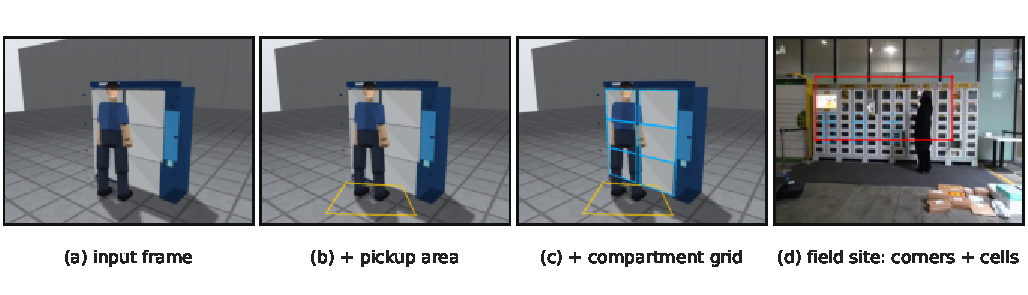
\includegraphics[width=0.98\textwidth]{figures/fig3_calibration.pdf}
\caption{One-time calibration, shown on the rendered scene and on field footage. (a)~the
reference frame; (b)~with the pickup-area polygon $P$ drawn on the ground in front of the
bank; (c)~with the compartment grid generated by~\eqref{eq:grid} after the operator marks the
four panel corners; (d)~the same procedure applied to a real installation
(Section~\ref{sec:field}), with the marked corners and the resulting cells overlaid. Both
tools export normalized polygons, so the procedure is identical on the rendered benchmark
(Section~\ref{sec:setup}) and on real sites.\label{fig:calib}}
\end{figure}

\subsection{Detection, tracking and geometric guards}
\label{sec:tracking}
Person detection uses a COCO-pretrained lightweight detector at input size 480 and confidence
threshold 0.35~\cite{yolov8ultralytics}; when the deep runtime is unavailable the system
falls back to a HOG descriptor with a linear SVM~\cite{dalal2005hog}, replacing only the
detector and keeping all downstream logic identical. Both backends are exercised in the
experiments; the fallback is a degraded mode, not a substitute
(Section~\ref{sec:exp-det}).

Tracking is association-based, with three mechanisms whose parameters were set by measured
failure modes. Each detection $d$ is matched to the live track $\tau$ maximizing the
intersection-over-union
\begin{equation}
\label{eq:iou}
\mathrm{IoU}(d,\tau) \;=\;
\frac{|B(d)\cap B(\tau)|}{|B(d)\cup B(\tau)|}
\;\ge\; \theta_{\mathrm{iou}} = 0.30 ,
\end{equation}
where $B(\cdot)$ is the bounding box; matching is greedy in decreasing IoU and each track
accepts at most one detection per frame. Stage two re-associates the unmatched detections:
a detection joins a recent track whose foot point is the nearest within radius
$\rho_{\mathrm{reid}}=45$~px, provided the track's age does not exceed
$\tau_{\mathrm{reid}}=12$~s. The need for stage two is empirical: on the rendered benchmark,
standing persons are intermittently missed by the detector for \mbox{4.1--10.5}~s, and
without re-association one physical person fragments into several tracks, resetting
accumulated presence and destroying the predicates of \eqref{eq:ev-loit}
(Section~\ref{sec:exp-abl}). The radius is bounded by the geometry of the scene: a person
walking across the campus scene moves at most about $120$~px/s at the working distance, so
$45$~px covers the worst-case displacement during a detection gap only if the gap is short;
therefore the radius is deliberately conservative (favour splitting over merging),
and the long-gap case is handled by track age alone, where the two-tracks risk of merging is
negligible because the arrival interval between different persons at the bank is much longer
than the allowed re-association windows.

Two guards protect the association against \emph{partial detections}---upper-body boxes that
the detector emits when a person bends towards a compartment. Both operate on the principle
that a partial box moves the foot point spuriously: its bottom edge sits mid-frame rather
than at the person's feet. The first guard compares the foot-point displacement between
consecutive accepted detections against a speed bound:
\begin{equation}
\label{eq:jump}
\bigl\|\phi_t-\phi_{t'}\bigr\|_2 \;>\; v_{\max}\,(t-t') + b,
\qquad v_{\max}=150~\mathrm{px/s},\;\; b=40~\mathrm{px},
\end{equation}
where $\phi_{t'}$ is the previously trusted foot point; the second guard is a box-height
test against the track's trusted height,
\begin{equation}
\label{eq:height}
h_t \;<\; \rho_h\,\hat{h}, \qquad \rho_h = 0.70 ,
\end{equation}
matched to the measured geometry of partial boxes (an upper-body box retains roughly
$47$~\% of the full height on the benchmark, so $0.70$ separates the modes with margin while
leaving ordinary box-height variation---perspective and gait---admissible). When either guard
fires, the frame updates neither the trusted foot point nor the trusted height, and the zone
state is held rather than re-evaluated; Algorithm~\ref{alg:assoc} states the complete
procedure. The guards are pure functions with unit tests, and their contributions are
isolated by the ablation (Section~\ref{sec:exp-abl}).

\begin{algorithm}[H]
\caption{Two-stage track association with geometric guards (per frame).}
\label{alg:assoc}
\begin{algorithmic}[1]
\Require detections $D_t$; live tracks $\mathcal{T}$; thresholds $\theta_{\mathrm{iou}},
\tau_{\mathrm{ttl}}, \tau_{\mathrm{reid}}, \rho_{\mathrm{reid}}, v_{\max}, b, \rho_h$
\Ensure association pairs; updated track set
\State $\mathcal{L} \gets \{\tau \in \mathcal{T} : t-\tau_{last} \le \tau_{\mathrm{ttl}}\}$
\State match $\mathcal{L} \times D_t$ greedily by \eqref{eq:iou} \Comment{stage 1: IoU}
\ForAll{unmatched $d \in D_t$}
  \State $\mathcal{C} \gets \{\tau \notin \text{matched}: 0 < t-\tau_{last} \le
    \tau_{\mathrm{reid}} \;\wedge\; \|\phi(d)-\phi(\tau)\| \le \rho_{\mathrm{reid}}\}$
  \If{$\mathcal{C} \neq \emptyset$} associate $d$ with the nearest track in $\mathcal{C}$
      \Comment{stage 2: re-association}
  \EndIf
\EndFor
\State create a new track for every still-unmatched detection
\State drop tracks with $t-\tau_{last} > \tau_{\mathrm{reid}}$; mark guarded frames per
       \eqref{eq:jump}--\eqref{eq:height}
\end{algorithmic}
\end{algorithm}

\subsection{Per-compartment door state}
\label{sec:door}
The open/closed state of compartment $k$ is estimated from its visual appearance, because no
per-door sensor exists at the target installations. The estimator rests on one contrast
observation: when a door is closed, the region shows the \emph{reflective door panel}; when it
is open, the region exposes the \emph{dark interior}. Let $\gamma(\mathbf{x})$ be the
grayscale value of pixel $\mathbf{x}$ in frame $v_t$ and $m=\mathrm{median}_{\mathbf{x}}
\gamma(\mathbf{x})$ the frame median, which tracks global illumination changes. Define the
dark indicator and the darkness ratio of $C_k$ as
\begin{equation}
\label{eq:dark}
I(\mathbf{x}) = \mathbbm{1}\bigl[\gamma(\mathbf{x}) < \kappa\, m\bigr],
\qquad
r_k(t) \;=\; \frac{1}{|C_k^{\mathrm{vis}}|}
\sum_{\mathbf{x}\in C_k^{\mathrm{vis}}} I(\mathbf{x}),
\qquad \kappa = 0.62,
\end{equation}
where $C_k^{\mathrm{vis}} = C_k \setminus \bigcup_{\tau} B(\tau)$ excludes pixels covered by
current or recent person boxes (occlusion masking). Following the design of
Section~\ref{sec:events}, the state decision is
\begin{equation}
\label{eq:door-decision}
\hat{d}_k(t) =
\begin{cases}
\text{open} & r_k(t) \ge \eta, \quad \eta = 0.15,\\[2pt]
\text{closed} & \text{otherwise,}
\end{cases}
\qquad\text{provided}\quad
\nu_k(t) \;=\; \frac{|C_k^{\mathrm{vis}}|}{|C_k|} \;\ge\; \nu_{\min} = 0.50;
\end{equation}
when the visibility condition fails, the estimator returns \emph{unknown} and the state
machine holds the previous value rather than guessing.

Why this decision rule is well-posed can be seen from a two-population model. Suppose that,
conditioned on the door state, the pixels of $C_k^{\mathrm{vis}}$ are drawn independently
from distributions with dark-pixel probabilities $\varepsilon_c$ (closed) and
$\varepsilon_o$ (open), $\varepsilon_c < \varepsilon_o$. Then $r_k$ is the mean of
$n_k=|C_k^{\mathrm{vis}}|$ Bernoulli variables with $\mathbb{E}[r_k\mid \text{closed}] =
\varepsilon_c$ and $\mathbb{E}[r_k\mid \text{open}] = \varepsilon_o$; the threshold $\eta$
separates the states whenever $\varepsilon_c < \eta \le \varepsilon_o$. The probability of a
false ``open'' decision on a closed compartment obeys the Chernoff bound
\begin{equation}
\label{eq:chernoff}
\Pr\bigl[r_k \ge \eta \,\big|\, \text{closed}\bigr]
\;\le\; \exp\bigl(-n_k\, D(\eta\,\|\,\varepsilon_c)\bigr),
\qquad
D(a\|b) = a\ln\frac{a}{b} + (1-a)\ln\frac{1-a}{1-b}.
\end{equation}
With the field measurements of Section~\ref{sec:field} ($\varepsilon_c \approx 0.07$ for a
real closed door including its edge pixels, $\eta=0.15$) and a compartment of about
$10^3$ visible pixels, the bound gives a false-open probability below $10^{-15}$ per frame;
the empirical margins are much wider still ($\varepsilon_c \le 0.07$ and
$\varepsilon_o \approx 0.94$ on the measured episode), which is what makes a single global
$\eta$ defensible across doors and brands. Two practical caveats bound this argument. Pixel
independence is an approximation---door edges and shadows correlate neighbouring pixels, so
the bound is indicative rather than exact; and the model presumes that \emph{closed} means
``reflective door panel'', which fails on lockers whose doors carry large dark viewing
windows. The audit of Section~\ref{sec:audit} therefore includes a per-site check of
$\varepsilon_c$, and Section~\ref{sec:field} reports a real installation where this
assumption needed recalibration. Finally, none of the door decisions is a measurement of
door angle: $\hat{d}_k$ is a binary proxy, which bounds the
interpretation of every door-related metric.

The estimator's remaining design choices address the three failure modes we measured.
(i) Occlusion: person pixels are excluded as in \eqref{eq:dark}, and when more than half of
$C_k$ is covered the state is undecidable and held---the system prefers abstention to a
guess. The look-back window that defines ``recent'' person boxes is short
($1.0$~s of recent track boxes) because a longer window lets the residual boxes of persons
who already left keep occluding a compartment, freezing its state and causing missed door
alarms, an effect we observed during development and fixed by shortening the window.
(ii) Brightness drift: the ratio is computed against the frame median, which cancels
smooth global changes such as dusk or cloud cover; abrupt changes (a light switched on) do
not move the decision because both the reference and the compartments brighten together.
(iii) Partial boxes: guarded by \eqref{eq:jump}--\eqref{eq:height} at the tracking stage,
so the estimator is never handed a mid-frame foot point as if it were a person standing
still. Algorithm~\ref{alg:door} states the per-compartment procedure and its flag state
machine; the flag itself (set at $\tau_{\mathrm{open}}$, cleared after
$\tau_{\mathrm{close}}$ of consistent closed evidence) is a hysteresis element, and its two
timers are the only door-related state.

\begin{algorithm}[H]
\caption{Per-compartment door state and flag state machine (per frame).}
\label{alg:door}
\begin{algorithmic}[1]
\Require frame $v_t$; compartment polygons $\{C_k\}$; recent track boxes; thresholds
$\kappa, \eta, \nu_{\min}, \tau_{\mathrm{open}}, \tau_{\mathrm{close}}$
\Ensure door states; door events
\ForAll{compartments $k$}
  \If{$\nu_k(t) < \nu_{\min}$} hold state($k$) \Comment{occlusion compensation}
  \Else
    \State $r_k \gets$ darkness ratio \eqref{eq:dark}; $\hat{d}_k \gets$ decision
           \eqref{eq:door-decision}
  \EndIf
  \If{$\hat{d}_k = \text{open}$} $T^{\mathrm{open}}_k \mathrel{+}= \Delta t$; reset
      $T^{\mathrm{closed}}_k$ \Else\ $T^{\mathrm{closed}}_k \mathrel{+}= \Delta t$; reset
      $T^{\mathrm{open}}_k$ \EndIf
  \If{$f_k=0$ \textbf{and} $T^{\mathrm{open}}_k \ge \tau_{\mathrm{open}}$} $f_k \gets 1$;
      emit \emph{DoorLeftOpen}($k$)
  \EndIf
  \If{$f_k=1$ \textbf{and} $T^{\mathrm{closed}}_k \ge \tau_{\mathrm{close}}$} $f_k \gets 0$;
      emit \emph{DoorClosed}($k$)
  \EndIf
\EndFor
\end{algorithmic}
\end{algorithm}

\subsection{Handheld package counting}
\label{sec:packages}
The evidence for retrieval events is a count of package-like objects associated with each
track. Package-like objects are connected components of a fixed colour-domain mask in HSV
space (hue within $[15,95]$, saturation $\ge 130$, value $\ge 90$, area within
$[60,1200]$~px), a proxy calibrated on the target domain (food containers and delivery bags
in warm tones). A blob counts as \emph{carried} by track $\tau$ when its centre falls inside
the box of $\tau$ expanded horizontally by $35\%$ and vertically by $15\%$; the expansion is
required because a package borne with an outstretched arm lies outside the detector's box,
and the guard on the expansion excludes regions that overlap a compartment polygon, so that
packages resting on the shelf are not counted as carried. Adjacent blobs of different
package colours (gap $\le 10$~px) are merged into one package. The predicate of
\eqref{eq:ev-multi} then fires when the count reaches $n_{\mathrm{multi}}=2$. Because the
mask is a colour proxy, its domain assumptions are checked at installation by the audit of
Section~\ref{sec:audit}, and its behaviour on field footage is quantified in
Section~\ref{sec:field}.

\subsection{Rule engine, event algebra and latency}
\label{sec:rules}
The rule engine consumes $\{o_t\}$ and maintains, per track, the zone state with a two-frame
debounce, accumulated nearby time, entry count, longest single visit and the set of fired
events; per compartment, the flag $f_k$ and the two timers of Algorithm~\ref{alg:door}. One
step of the engine realizes the predicates \eqref{eq:ev-door}--\eqref{eq:ev-loit} and the
cooldown; the complete procedure is Algorithm~\ref{alg:rules}. Two properties of the engine
make the system auditable in an operational sense.

\emph{Alarm latency is predictable.} Consider the door alarm \eqref{eq:ev-door}. The
accumulator $T^{\mathrm{open}}_k$ advances only while the estimator reports ``open'', so if
compartment $k$ is opened at time $t_0$ and the estimator reports the first ``open'' at
$t_0+\delta$ (the detection delay), the alarm time is
\begin{equation}
\label{eq:latency}
t_{\mathrm{alarm}}(k) \;=\; t_0 + \delta + \tau_{\mathrm{open}},
\end{equation}
provided the compartment stays open throughout. On the benchmark, the measured alarm times
sit at $14.1$--$16.3$~s in clips whose doors open in the first seconds, consistent
with~\eqref{eq:latency} at $\tau_{\mathrm{open}}=10$~s and $\delta$ of order the detection
period; more importantly, the same identity makes threshold changes \emph{replayable}: the
opening time is recoverable from the recorded alarm as $t_0 = t_{\mathrm{alarm}} -
\tau_{\mathrm{open}} - \delta$, and every statement about a different threshold can be
derived without re-running video. Section~\ref{sec:replay} turns this into a method and
verifies it against the measured counts.

\emph{Cooldown is keyed and counted.} Suppression is keyed by (event type, target), so a
repeated alarm for the same door waits $\tau_{\mathrm{cool}}$ while an alarm for a different
door passes immediately; the number of suppressed events is exposed as a first-class
statistic. During the benchmark evaluation the cooldown suppressed 299 repeated firings over
29\,190 processed frames---without it, ongoing situations (a door still open) would flood the
event log, and with it the log remains a faithful record of distinct situations.

\begin{algorithm}[H]
\caption{Behaviour rule engine (per frame).}
\label{alg:rules}
\begin{algorithmic}[1]
\Require observation $o_t$; time $t$; configuration
\Ensure event list
\State associate detections to tracks (Algorithm~\ref{alg:assoc}); update zone with a
       $\zeta$-frame debounce per \eqref{eq:zone}
\State \textbf{if} debounced zone entry \textbf{and} cooldown ok \textbf{then} emit
       \emph{PickupEntry}
\State \textbf{if} $L_\tau \ge \tau_{\mathrm{loit}}$ \textbf{and}
       $e_\tau \ge n_{\mathrm{entries}}$ \textbf{and}
       $\mu_\tau < \tau_{\mathrm{peak}}$ \textbf{and} not yet fired \textbf{then} emit
       \emph{Loitering}
\State update door states and flags (Algorithm~\ref{alg:door}) and emit door events
\State \textbf{if} $c_\tau \ge n_{\mathrm{multi}}$ and cooldown ok \textbf{then} emit
       \emph{MultiRetrieval}
\State \textbf{if} $f_k=1$ and $n_k$ decreases \textbf{and} cooldown ok \textbf{then} emit
       \emph{FlaggedRetrieval}($k$)
\State suppress repeats per (type, target) within $\tau_{\mathrm{cool}}$; count suppressions
\end{algorithmic}
\end{algorithm}

\subsection{Analytic replay of threshold sensitivity}
\label{sec:replay}
Because the alarms are threshold predicates over recorded quantities, their sensitivity to a
parameter does not require re-running any video. We use this in two ways: as a method, to
characterize the usable range of the door threshold at zero cost, and as a self-check, by
verifying that the replay reproduces the measured counts at the deployed value.

For each door event recorded in an evaluation run, let $t_{\mathrm{alarm}}$ be its alarm
time; by \eqref{eq:latency} the (estimated) opening instant is
\begin{equation}
\label{eq:replay-open}
\hat{t}_0 \;=\; t_{\mathrm{alarm}} - \tau_{\mathrm{open}} - \delta,
\end{equation}
with $\delta$ the mean detection delay, and let $A_k$ be the available open duration of the
compartment---the time from $\hat{t}_0$ until the compartment is confirmed closed, or until
the clip ends. Under an alternative threshold $\tau'$, the door alarm fires iff the
compartment remains open for that long, and the derived flagged-retrieval alarm fires iff,
additionally, the package is taken \emph{after} the flag is raised. Writing the recorded
retrieval instant as $t_{\mathrm{take}}$, the replay computes
\begin{align}
R_{\mathrm{door}}(\tau') &= \frac{1}{N}\sum_{k}
   \mathbbm{1}\bigl[A_k \ge \tau'\bigr],
\label{eq:replay-door}\\[2pt]
R_{\mathrm{flag}}(\tau') &= \frac{1}{N}\sum_{k}
   \mathbbm{1}\bigl[A_k \ge \tau' \;\wedge\;
   t_{\mathrm{take}} \ge \hat{t}_0 + \tau'\bigr],
\label{eq:replay-flag}
\end{align}
over the $N$ door events of the recording. Both formulas are exact under two stated
assumptions---the open interval is contiguous (no re-opening), and $\delta$ is constant
across clips---which hold on the benchmark and can be checked per event from the recorded
timeline. The verifications and the resulting operating recommendations are reported in
Section~\ref{sec:exp-sens}; the same mechanism is what makes the field episode of
Section~\ref{sec:field-door} interpretable against the deployed threshold.

\subsection{Computational cost model}
\label{sec:cost}
All per-frame work beyond detection is linear in the number of persons and compartments. The
association is $O(|\mathcal{L}||\mathcal{D}_t|)$ in the worst case but runs with one to three
tracks in practice; the package mask is one HSV threshold plus connected components; the door
estimator reads only compartment pixels, which cover about $13\%$ of a $640\times480$ frame
for the six-compartment layout. Writing $T_{\mathrm{det}}$ for per-frame detection cost and
$T_{\mathrm{obs}}$ for the complete observation step, the sustained detection rate of one
view is
\begin{equation}
\label{eq:costmodel}
f_{\mathrm{det}} \;=\; \frac{1}{T_{\mathrm{det}}+T_{\mathrm{obs}}},
\qquad
N_{\mathrm{views}} \;\le\; \frac{1}{f_s\,(T_{\mathrm{det}}+T_{\mathrm{obs}})}
\end{equation}
for an $f_s$-frame-per-second source: the number of views one machine can monitor at frame
rate is bounded by the same budget, which turns ``one machine suffices'' into a measured
inequality rather than a slogan. Section~\ref{sec:exp-cost} reports the measured terms and
the implied envelope, including the multi-view limit that this economy does \emph{not}
reach.
%%%%%%%%%%%%%%%%%%%%%%%%%%%%%%%%%%%%%%%%%%
\section{Experimental Setup}
\label{sec:setup}

\subsection{Hardware, software and fixed configuration}
\label{sec:exp-setup}
All experiments ran on a single personal computer with an Intel Core i5-12500H
(16 logical cores) and 15.7~GB of RAM under Windows~11, using Python 3.13.9,
PyTorch 2.14.0+cpu, Ultralytics 8.4.161, OpenCV 4.12.0 and Flask 3.1.3. Inference is
CPU-only; input is always a local video file. Unless stated otherwise, the detector runs at
input size 480 with confidence threshold 0.35 and IoU threshold 0.50, and the rule
parameters are the defaults of Table~\ref{tab:params}. The system, its calibration tools
and the evaluation scripts are the same code base that serves the operator console.

\begin{table}[H]
\caption{Default configuration. Every entry is a named parameter of the configuration
object rather than a constant in the code; the defaults below are those used in all
experiments unless explicitly varied.\label{tab:params}}
\small
\begin{tabularx}{\textwidth}{l l X}
\toprule
\textbf{Group} & \textbf{Parameter} & \textbf{Value} \\
\midrule
Detection & confidence threshold & 0.35 \\
 & IoU threshold / input size & 0.50 / 480 \\
 & HOG input width & 320~px \\
\midrule
Tracking & IoU match threshold $\theta_{\mathrm{iou}}$ & 0.30 \\
 & short track TTL $\tau_{\mathrm{ttl}}$ & 3.0~s \\
 & re-association TTL $\tau_{\mathrm{reid}}$ & 12.0~s \\
 & re-association radius $\rho_{\mathrm{reid}}$ & 45~px \\
 & foot-speed guard $v_{\max}$ / margin $b$ & 150~px/s / 40~px \\
 & box-height ratio guard $\rho_h$ & 0.70 \\
 & zone debounce $\zeta$ & 2 frames \\
\midrule
Door state & median factor $\kappa$ / open threshold $\eta$ & 0.62 / 0.15 \\
 & minimum visibility $\nu_{\min}$ & 0.50 \\
 & occlusion look-back & 1.0~s \\
\midrule
Rules & door-open alarm $\tau_{\mathrm{open}}$ & 10~s \\
 & close confirmation $\tau_{\mathrm{close}}$ & 1.5~s \\
 & multi-package count $n_{\mathrm{multi}}$ & 2 \\
 & loitering $\tau_{\mathrm{loit}}$ / $n_{\mathrm{entries}}$ & 15~s / 3 \\
 & single-visit peak $\tau_{\mathrm{peak}}$ & 8~s \\
 & compartment proximity factor & $\times 1.45$ \\
 & event cooldown $\tau_{\mathrm{cool}}$ & 30~s \\
\midrule
Runtime & display / detect rate & 30 / 15~fps \\
\bottomrule
\end{tabularx}
\end{table}

\subsection{Rendered behaviour benchmark}
\label{sec:bench}
The behaviour benchmark consists of 119 clips (84 abnormal, 35 normal) rendered as
640$\times$480 videos at 15~fps, 10--22~s per clip (29\,190 frames). This sample size
bounds the resolution of every rate reported below: Wilson 95\% intervals are 96.9--100\%
for the 119 clips, 90.1--100\% for the 35 normal clips and 91.6--100\% for the 42 door
events, while a 0/21 outcome excludes recall above 15.5\% rather than establishing it at zero. The abnormal half
covers four event classes with 21 clips each: door left open, multiple packages by one
person, retrieval from a flagged compartment, and loitering; the normal half contains
complete retrievals. The clips are produced by a scripted three-dimensional scene
generator that renders the locker with the compartment layout used by the calibration
(Figure~\ref{fig:calib}) together with scripted human trajectories and package placements;
ground truth---per-compartment door angle, retrieval instants and the expected event type of
every clip---is exported programmatically, so the evaluation involves no manual annotation.
Because the test scene, the calibration and the renderer are consistent, results on this
benchmark verify \emph{correctness under same-distribution conditions}: that the
implementation executes the specified decision procedure and that the declared thresholds
behave as intended. They are not, and are not used as, an estimate of generalization to
unseen scenes.

The accompanying survey referenced throughout the paper was conducted by the project team
among campus locker users: 130 questionnaires were distributed and 120 valid responses were
recovered (92.3\%). The response pattern---86.7\% perceiving security risks in current
locker use, 91.7\% supporting automated behaviour recognition, 88.3\% requiring
non-intrusive supervision and 74.2\% concerned about low illumination (Wilson 95\% CIs at
$n=120$: 79.4--91.6, 85.3--95.4, 81.4--92.9 and 65.7--81.2\%, respectively; questionnaire
recovery 120 of 130, 95\% CI 86.4--95.8)---motivated the
requirements of Section~\ref{sec:intro} and is reported here so that the event vocabulary
and the operating constraints can be traced to their origin.

\subsection{Real-image detector benchmark}
\label{sec:exp-det}
To anchor the detector comparison on real photographs rather than rendered scenes, the
backends are evaluated on a fixed 500-image subset of the COCO val2017 person class~\cite{lin2014coco} (400
images containing persons plus 100 without; 1670 ground-truth boxes; fixed sampling seed
20260925, manifest stored with the evaluation logs). Metrics are average precision at IoU
0.5 (VOC all-point interpolation, greedy matching, crowd annotations excluded) and
precision/recall/F1 at the operating confidence 0.35, together with single-image inference
time measured on the deployment machine after a warm-up pass. Three backends are compared:
YOLOv8n, its successor YOLO11n~\cite{reveles2025yolo11}, and the HOG+SVM
fallback~\cite{dalal2005hog}.

\subsection{Real surveillance footage}
\label{sec:avenue}
As an additional real-domain probe, the complete pipeline (detection, observations, rules,
event emission) runs over all 15\,328 frames of the 16 CUHK Avenue training sequences~\cite{lu2013avenue}---a
real scene with no relation to the locker geometry. This experiment is deliberately
reported as a boundary study, not as an accuracy metric: without calibration the geometric
rules are meaningless by construction, and the quantity of interest is how unusable an
uncalibrated deployment is in practice (Section~\ref{sec:exp-cross}).

\subsection{Field corpus}
\label{sec:field-corpus}
The field corpus consists of 15 publicly available recordings of real locker use, gathered
from video-sharing platforms to represent the deployment domain as it actually exists. In
total 19.1~min of footage (1145~s) covering at least six distinct physical installations:
a campus locker bank at Fudan University (several clips), a static campus bank used for meal
storage and retrieval, a campus deployment at Changshu
Institute of Technology, a Fengchao express-locker site, an indoor food-locker room, an
Xintian smart-cabinet deployment, a canteen pickup cabinet at a university west building,
and a campus deployment at a college in Wuhu; the corpus also includes three vendor
demonstration clips and one television report on contactless pickup. The recordings differ
in resolution (640$\times$368 to 1280$\times$720), aspect ratio (landscape and portrait),
camera motion (static surveillance-style framing to handheld close-ups), and illumination
(outdoor daytime to artificially lit interiors at night). Table~\ref{tab:field} summarizes
the corpus; per-frame statistics (brightness, motion) and per-site audit quantities are
reported there because they matter for both the transfer results
(Section~\ref{sec:field}) and the audit procedure (Section~\ref{sec:audit}).

The recordings are used exclusively as footage---they are fed to the pipeline as inputs,
not redistributed---and the paper reports only aggregate statistics and a small number of
frames as qualitative evidence, with the source recordings identified in the data
availability statement. No personal identifying information is analyzed; the recordings are
public, and the analysis is limited to gross behaviour (presence, door state, carried
objects).

\begin{table}[H]
\caption{Field corpus. One row per recording (sorted as processed); \emph{motion} is the
median inter-frame difference within a mid-clip window in 8-bit grey levels
(higher = more camera/global motion),
\emph{collision} is the colour-domain audit of Section~\ref{sec:audit} (fraction of
person-frames in which at least two package-coloured blobs fall inside a person box), and
\emph{events} is the number of events emitted by the uncalibrated configuration of
Section~\ref{sec:field-transfer} (informational and alarm events combined; 197 of the 261
are alarms).\label{tab:field}}
\small
\setlength{\tabcolsep}{3pt}
\begin{tabularx}{\textwidth}{l X r r r r r}
\toprule
\textbf{ID} & \textbf{Scene (abbreviated)} & \textbf{Dur (s)} & \textbf{Resolution} & \textbf{Motion} & \textbf{Collision} & \textbf{Events} \\
\midrule
v01 & Fudan campus, courier deposit & 45.9 & 852$\times$480 & 2.02 & 55.4\% & 20 \\
v02 & Fudan campus, pickup & 32.7 & 852$\times$480 & 11.11 & 39.3\% & 4 \\
v03 & Fudan campus, courier deposit (long) & 318.6 & 852$\times$480 & 9.09 & 48.3\% & 74 \\
v04 & Campus bank, storage/retrieval (static) & 240.3 & 852$\times$480 & 0.61 & 6.9\% & 48 \\
v05 & Fengchao express, door-closing clip & 50.0 & 1280$\times$720 & 1.23 & 46.9\% & 10 \\
v06 & Food locker, close-up clip & 26.9 & 854$\times$474 & 4.66 & 11.1\% & 1 \\
v07 & Indoor locker room, multi-user & 88.4 & 1280$\times$720 & 4.14 & 30.1\% & 24 \\
v08 & Changshu campus deployment & 31.8 & 1280$\times$720 & 4.74 & 41.7\% & 5 \\
v09 & Xintian smart cabinet, usage flow & 56.8 & 640$\times$368 & 3.07 & 19.0\% & 6 \\
v10 & Express locker, vendor demo (portrait) & 24.4 & 720$\times$1280 & 0.63 & 47.6\% & 7 \\
v11 & TV report, contactless pickup & 84.1 & 1280$\times$720 & 5.03 & 29.9\% & 44 \\
v12 & Handover cabinet, vendor demo & 21.1 & 1280$\times$720 & 8.32 & 0.0\% & 0 \\
v13 & Express locker, vendor demo & 59.5 & 720$\times$720 & 2.96 & 50.0\% & 8 \\
v14 & Wuhu college deployment & 17.8 & 720$\times$1280 & 1.96 & 66.7\% & 4 \\
v15 & Canteen pickup cabinet & 46.5 & 1280$\times$720 & 2.28 & 43.6\% & 6 \\
\midrule
 & \textbf{Total} & \textbf{1144.8} & --- & --- & \textbf{28.3\%} & \textbf{261} \\
\bottomrule
\end{tabularx}
\end{table}

%%%%%%%%%%%%%%%%%%%%%%%%%%%%%%%%%%%%%%%%%%
\section{Controlled Experiments}
\label{sec:experiments}

\subsection{Behaviour-level evaluation on the rendered benchmark}
\label{sec:exp-e1}
A first question the benchmark must answer is \emph{where the system's behaviour actually
lives}: does the alarm semantics come from the detector, or from the rules on top of it?
Comparing the complete pipeline against a detector-only baseline and against a
HOG-based fallback answers it directly. Arm A1 applies the detector alone (a clip is
predicted abnormal if a person is detected in any frame); A2 is the complete pipeline; A3
replaces the deep detector with the HOG fallback while keeping every rule and threshold
identical. Table~\ref{tab:e1} and Figure~\ref{fig:e1} show the outcome, and it is
unambiguous: the detector contributes presence, the rules contribute meaning.

\begin{table}[H]
\caption{Clip-level results of the three arms on the 119-clip behaviour benchmark
(84 abnormal / 35 normal; confusion counts in TP/FP/FN/TN order, A1 84/35/0/0,
A2 84/0/0/35, A3 60/0/24/35).\label{tab:e1}}
\small
\begin{tabularx}{\textwidth}{l C C C C}
\toprule
\textbf{Arm} & \textbf{Precision} & \textbf{Recall} & \textbf{F1} & \textbf{Accuracy} \\
\midrule
A1: detector only & 0.706 & 1.000 & 0.828 & 0.706 \\
A2: YOLOv8n + rules & \textbf{1.000} & \textbf{1.000} & \textbf{1.000} & \textbf{1.000} \\
A3: HOG + rules & 1.000 & 0.714 & 0.833 & 0.798 \\
\bottomrule
\end{tabularx}
\end{table}

The outcome separates the two contributions cleanly. The detector alone already recovers
every abnormal clip (recall 1.000), but it also flags all 35 normal retrievals, since a
person appears in every one of them; its clip-level precision is therefore only 0.706.
Adding the rule engine removes exactly these false positives and lifts the complete
pipeline to precision, recall and F1 of 1.000---the behaviour semantics evidently come from
the rules rather than from the detector. The HOG fallback tells a complementary story:
sharing the same rules, it preserves a precision of 1.000---it never raises an alarm on a
normal clip---but misses 24 of the 84 abnormal clips (recall 0.714). For an alarm system
this is the correct failure mode of a degraded backend: silence is preferable to noise,
which is why HOG is positioned as a fallback rather than a substitute. The 24 misses are
not scattered: they are exactly the 21 multiple-package clips and 3 of the 21 loitering
clips---the classes that require locating people and their carried packages.

Event-level scoring sharpens where the fallback breaks (Table~\ref{tab:e2ev}). With YOLOv8n every expected event
of all four classes is detected: 42/42 door-left-open events across the two door-related
classes and 21/21 in each of the others, with micro and macro P/R/F1 all 1.000. Under
HOG, door-left-open events remain perfect, because that judgment reads compartment
appearance rather than people, and loitering degrades only modestly (18 of 21 detected,
6 spurious); but retrieval-from-flagged-door collapses to 1/21 and multiple-package to
0/21. The two views expose different failure surfaces: the substitution that costs a
third of the clips also removes two event classes almost entirely.

\begin{table}[H]
\caption{Event-level results of A2 and A3 on the benchmark. Micro P/R/F1: A2
1.000/1.000/1.000; A3 0.910/0.581/0.709.\label{tab:e2ev}}
\small
\setlength{\tabcolsep}{3pt}
\begin{tabularx}{\textwidth}{l CCC CCC}
\toprule
& \multicolumn{3}{c}{\textbf{A2 (YOLOv8n)}} & \multicolumn{3}{c}{\textbf{A3 (HOG)}} \\
\cmidrule(lr){2-4}\cmidrule(lr){5-7}
\textbf{Event} & TP & FP & FN & TP & FP & FN \\
\midrule
Door left open & 42 & 0 & 0 & 42 & 0 & 0 \\
Retrieval from flagged door & 21 & 0 & 0 & 1 & 0 & 20 \\
Multiple packages & 21 & 0 & 0 & 0 & 0 & 21 \\
Loitering & 21 & 0 & 0 & 18 & 6 & 3 \\
\bottomrule
\end{tabularx}
\end{table}

\begin{figure}[H]
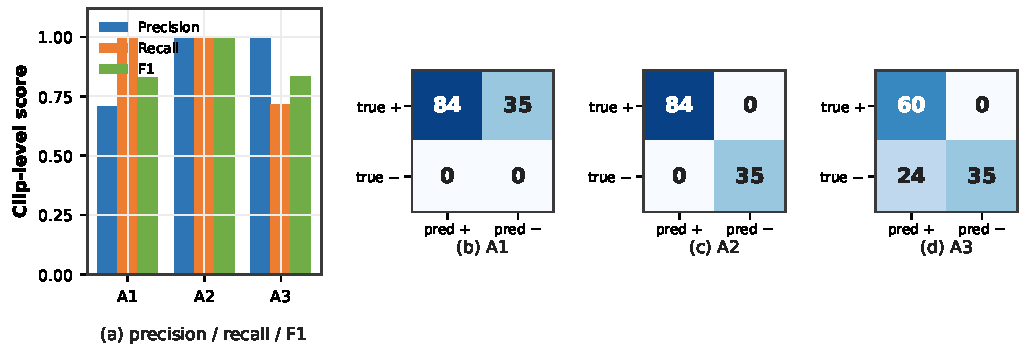
\includegraphics[width=0.98\textwidth]{figures/fig6_e1_arms.pdf}
\caption{Clip-level results of the three arms. Left: precision, recall and F1. Right:
confusion matrices (rows = true class). A1 confuses every normal clip with an abnormal one;
A2 is diagonal; A3 trades sensitivity for the same zero false-alarm
rate.\label{fig:e1}}
\end{figure}

The time structure of the alarms is itself a check of the design. On the benchmark, the
multiple-package rule---which carries no waiting threshold---fires as soon as the second
package becomes visible (7.5--7.7~s into the clip), while the two rules that wait fire at
latencies implied by their own thresholds: loitering at 15.0--15.3~s against its 15~s
accumulation threshold, and door-left-open at 14.1--16.3~s where the 10~s threshold applies
to the accumulated open time, consistent with \eqref{eq:latency}. In retrieval-from-flagged
clips the door alarm always precedes the retrieval alarm by 1.1--2.5~s (median 1.28~s), the
delay between flagging the compartment and the package leaving it. A rule therefore does
not fire at an arbitrary frame: its latency is the threshold it declares plus the detection
delay, which is what makes the alarms auditable in time as well as in quantity.

\subsection{A second, cross-scene rendered set}
\label{sec:exp-variant}
A perfect score on the benchmark of Section~\ref{sec:exp-e1} is a statement about the
implementation, not about generalization: the clips were rendered by the same scene
generator whose calibrated geometry the pipeline uses. To test what survives when that
self-consistency is removed, we rendered a second set with the same behavioural
scripts but under a different camera pose and field of view (eye moved from
$(2.35,1.92,-3.25)$ to $(1.05,2.30,-2.60)$, FOV $48^\circ\!\to\!62^\circ$) and different
illumination (key light re-aimed, intensity $0.78\!\to\!0.60$, ambient $0.34\!\to\!0.46$),
and---the decisive step---re-calibrated the compartment polygons and pickup region
\emph{for that view} before evaluating, so the measurement tests the rules rather than a
stale geometry. The set contains 20 clips (16 abnormal, four normal).

The door statistic transfers cleanly under the new view: on the re-calibrated cells the
closed-state maximum is $0.024$ against an open-state minimum of $0.277$ (separation
$+0.254$), with all six compartments correctly assigned and no false ``open'' reading at
the deployed $\eta=0.15$. At the pipeline level the geometry- and state-machine-based
rules transfer without per-scene tuning---door-left-open is detected on 8 of 8 expected
clips, loitering on 4 of 4, and retrieval-from-flagged-compartment on 3 of 4---giving an
event-level micro $P=1.000$, $R=0.750$, $F_1=0.857$; twelve of the sixteen abnormal
clips are flagged and none of the four normal clips is false-alarmed (binary clip-level accuracy
$0.800$), while 15 of the 20 clips are fully correct at the per-event level. The failure
is specific and instructive: the multiple-package rule, which rests on the package colour
proxy rather than on geometry, fires on none of its four clips. The appearance-based
proxy that the collision audit of Section~\ref{sec:audit} exists to measure is exactly
the component that fails across the scene change, while the geometry-anchored components
survive once the geometry is re-calibrated. This is the intended reading of the
calibration-first design---the rules do not generalize for free, but they generalize
exactly where their assumptions hold, and the assumption that breaks is the one the
pre-deployment audit is built to test.

\subsection{Detector benchmark on real images}
\label{sec:exp-e2}
The detector choice at the edge is a design decision, not a tuning detail: inference must
share a CPU with the rest of the pipeline, so the smallest model of a current family is
the natural candidate, and it must be checked on real photographs rather than rendered
scenes. Both nano-scale generations clear the accuracy bar for this application, and the
HOG fallback does not come close. On the 500-image COCO subset~\cite{lin2014coco} (Table~\ref{tab:e3},
Figure~\ref{fig:e2}) YOLOv8n achieves AP@0.5 of 0.514
with a balanced operating point at the deployed confidence (P=0.896, R=0.525, F1=0.662);
YOLO11n performs comparably in accuracy (AP@0.5 0.494, F1 0.646) at essentially the same
CPU cost (median 26.9~ms versus 26.0~ms per image after a warm-up pass on an otherwise idle
machine; CPU-only timings are load-sensitive, so the same measurement taken under concurrent
load gave 28.4~ms and 66.5~ms respectively, which is why the idle figures are reported)---on
this CPU-only,
smallest-scale configuration the newer architecture's advantage is negligible, consistent
with benchmark studies that report marginal accuracy differences between recent YOLO
generations at the nano scale and attribute their differences mainly to training
behaviour~\cite{reveles2025yolo11}. We therefore keep YOLOv8n as the default and report
YOLO11n as a validated alternative. HOG is effectively non-functional on this benchmark
(AP@0.5 0.005, recall 0.019): its curve never leaves the leftmost 1.9\% of the recall axis,
whatever threshold it is given. This gap is the quantitative reason for the fallback
positioning---HOG keeps the pipeline alive when the deep runtime is unavailable, but it is
not a substitute.

\begin{table}[H]
\caption{Detector benchmark on 500 COCO val2017 images containing persons (1670
ground-truth boxes). AP is average precision at IoU 0.5; P/R/F1 are at the operating
confidence 0.35; inference time is the median per-image cost on the deployment machine
after a warm-up pass on an otherwise idle machine.\label{tab:e3}}
\small
\setlength{\tabcolsep}{4pt}
\begin{tabularx}{\textwidth}{l C C C}
\toprule
\textbf{Metric} & \textbf{YOLOv8n} & \textbf{YOLO11n} & \textbf{HOG + SVM} \\
\midrule
AP@0.5 & 0.5135 & 0.4942 & 0.0051 \\
Precision@0.35 & 0.8957 & 0.8941 & 0.2581 \\
Recall@0.35 & 0.5246 & 0.5054 & 0.0192 \\
F1@0.35 & 0.6616 & 0.6458 & 0.0357 \\
Median ms/image & 26.0 & 26.9 & 5.1 \\
\bottomrule
\end{tabularx}
\end{table}

\begin{figure}[H]
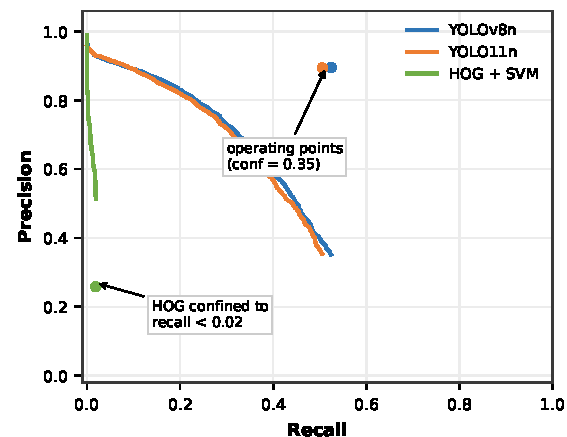
\includegraphics[width=0.98\textwidth]{figures/fig7_e2_pr.pdf}
\caption{Precision--recall curves on the COCO subset. The HOG curve is confined to the
leftmost 1.9\% of the recall axis; YOLOv8n and YOLO11n track each other closely, with
YOLOv8n holding a slight advantage at every operating point.\label{fig:e2}}
\end{figure}

\subsection{Real-time behaviour and the cost envelope}
\label{sec:exp-cost}
The budget question has a comfortable answer, and the cost structure behind it is the
reason the calibration-first design is affordable on a CPU. On the synthetic footage
(640$\times$480 at 15~fps) both backends process every frame in real
time ($\approx$14.9~fps for display and detection); on real surveillance video
(640$\times$360 at 25~fps) the display loop runs at $\approx$24~fps with either backend
while detection is throttled only by the configured interval (Table~\ref{tab:e4}).
Figure~\ref{fig:e3} decomposes why: the
detector alone accounts for about 24~ms (YOLOv8n) and 20~ms (HOG), whereas the complete
observation step---package colours and per-compartment door estimation included---adds
only a few milliseconds (27~ms and 22~ms totals). Everything downstream of detection is
therefore nearly free, which is exactly the property that lets the rule and audit layers
run beside inference; the frame budget of a 15~fps source is 66.7~ms, so the
measured totals leave headroom for the console and the persistence layer running beside the
pipeline.

Applying the cost model \eqref{eq:costmodel} to the measurements bounds the multi-view
envelope: at $T_{\mathrm{det}}+T_{\mathrm{obs}}\approx 27$~ms per frame, a single
machine sustains one 15--25~fps view comfortably but cannot serve three 25~fps views on
one process within the 40~ms budget (three views would need $\approx$81~ms). Scaling to
several locker banks per machine therefore requires the geometric cascade discussed in
Section~\ref{sec:discussion} or one process per view sharing an event store---both
compatible with the present design, neither implemented here.

\begin{table}[H]
\caption{Real-time behaviour on CPU (fps). The real-surveillance rows use the configured
detection interval (four frames for YOLOv8n, two for HOG).\label{tab:e4}}
\small
\setlength{\tabcolsep}{4pt}
\begin{tabularx}{\textwidth}{l C C C}
\toprule
\textbf{Source} & \textbf{Backend} & \textbf{Display} & \textbf{Detection} \\
\midrule
640$\times$480 @15~fps (synthetic) & YOLOv8n & 14.93 & 14.93 \\
 & HOG & 14.89 & 14.91 \\
640$\times$360 @25~fps (real) & YOLOv8n & 24.27 & 7.70 \\
 & HOG & 24.04 & 11.54 \\
\bottomrule
\end{tabularx}
\end{table}

\begin{figure}[H]
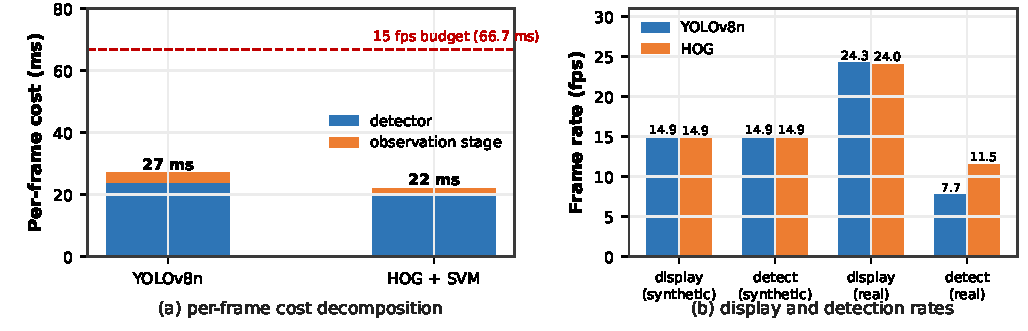
\includegraphics[width=0.98\textwidth]{figures/fig8_e3_cost.pdf}
\caption{(a)~Per-frame cost decomposition inside the processing process (640$\times$480
frames, $n=40$): detector alone and the complete observation step, against the 66.7~ms
frame budget of a 15~fps source; the HOG figure is measured with the deep-learning runtime
resident in the same process, and standalone it costs 5.1~ms per image (Table~\ref{tab:e3}).
(b)~measured display and detection rates for both backends on the synthetic and the real
source, i.e. the measurements tabulated in Table~\ref{tab:e4}.\label{fig:e3}}
\end{figure}

\subsection{Contribution of the failure-repair mechanisms}
\label{sec:exp-abl}
The ablation attributes the system's robustness to one mechanism above all others
(Table~\ref{tab:e5}, Figure~\ref{fig:ablation}). Over a
paired subset of 20 clips (four per behaviour class, four normal retrievals, one changed
parameter per row), removing the re-association stage costs all four loitering events and
turns four abnormal clips into misses (16 of 20 clips versus 12 of 20; Wilson 95\% CIs
58.4--91.9\% and 38.7--78.1\%), while leaving the door-related and
multiple-package classes untouched; the other three configurations are identical to the
complete system. The mechanism behind the number is directly observable: a person standing
motionless in front of a locker is missed by the detector for multi-second stretches, so
without re-association the track is destroyed, its accumulated presence resets, and the
15~s accumulation threshold is never reached. Door events survive the same ablation because
they depend on compartment appearance rather than track continuity---a deliberate property,
and one reason the door channel is the system's backbone.

Removing the occlusion look-back changes nothing on this subset; removing the partial-box
guards leaves detection unchanged but admits one spurious loitering event, which the
segment-level columns of Table~\ref{tab:e5} do not show. Both guards repair failure modes
associated with sustained stationary presence; when the
requirement analysis removed that class from the event vocabulary (a person waiting at a
locker is normal), the remaining 119 clips contain few instances that exercise these
guards. Their contribution is therefore not established by this ablation; what it does
establish is the converse and more useful fact: on footage without these failure modes the
guards can be disabled at zero cost, whereas re-association cannot. The occlusion policy
is nonetheless exercised in the field, where it turns a potentially misleading reading
into an explicit abstention (Section~\ref{sec:field-door}).

\begin{table}[H]
\caption{Ablation of the failure-repair mechanisms over 20 paired clips (segment-level
counts; correctly detected events out of the 20 expected, and event-level false positives,
which the segment columns conceal).\label{tab:e5}}
\small
\begin{tabularx}{\textwidth}{l C C C C C}
\toprule
\textbf{Configuration} & \textbf{Segment TP} & \textbf{Segment FP} & \textbf{Segment FN} & \textbf{Event TP} & \textbf{Event FP} \\
\midrule
Complete system & 16 & 0 & 0 & 20/20 & 0 \\
w/o re-association & 12 & 0 & 4 & 16/20 & 0 \\
w/o occlusion look-back & 16 & 0 & 0 & 20/20 & 0 \\
w/o partial-box guards & 16 & 0 & 0 & 20/20 & 1 \\
\bottomrule
\end{tabularx}
\end{table}

\begin{figure}[H]
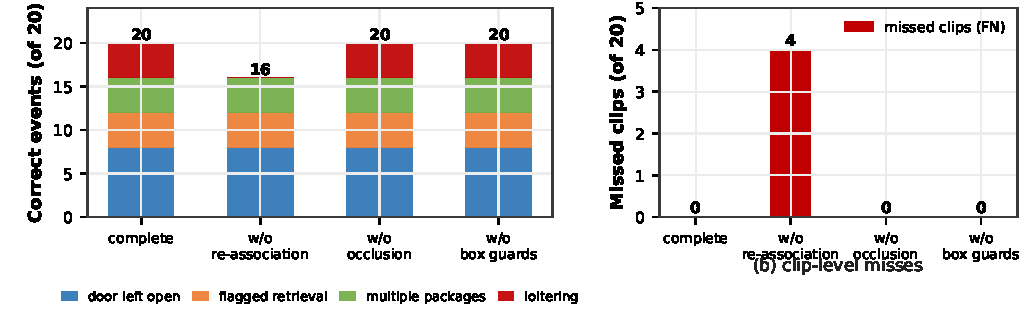
\includegraphics[width=0.98\textwidth]{figures/fig9_ablation.pdf}
\caption{Ablation over 20 clips. Left: correctly detected events per class. Right:
missed abnormal clips (FN) and false alarms (FP) at the clip level. Only the
re-association stage changes clip-level detection on this subset; the partial-box guards
add one event-level false positive, as discussed in the text.\label{fig:ablation}}
\end{figure}

\subsection{Threshold sensitivity by analytic replay}
\label{sec:exp-sens}
The replay of the recorded timelines turns the main threshold question into a direct,
derivable statement, and the answer is a usable range rather than a single value. Because
the alarm conditions are thresholds rather than learned parameters, the behaviour of the
119 clips under any door-open threshold $\tau'$ follows from their recorded timelines
without re-running a single video, via \eqref{eq:replay-open}--\eqref{eq:replay-flag}; at
the deployed value the replay reproduces the measured counts exactly
(42/42 door-left-open, 21/21 retrieval-from-flagged), which is what makes its
extrapolation a verification rather than a speculation (Table~\ref{tab:e6}).

\begin{table}[H]
\caption{Sensitivity to the door-open alarm threshold, obtained by replaying the recorded
timelines of the 119 clips. The 10~s row reproduces the measured counts
exactly.\label{tab:e6}}
\small
\begin{tabularx}{\textwidth}{l C C X}
\toprule
$\tau_{\mathrm{open}}$ & \textbf{Door left open} & \textbf{Flagged retrieval} & \textbf{Effect} \\
\midrule
5~s & 42/42 & 21/21 & earlier alarms only \\
\textbf{10~s (default)} & \textbf{42/42} & \textbf{21/21} & as measured \\
15~s & 42/42 & 0/21 & retrieval events lost \\
20~s & 0/42 & 0/21 & door events lost \\
\bottomrule
\end{tabularx}
\end{table}

Three regimes appear (Figure~\ref{fig:e10}). Below the deployed value both event types keep
recall 1.000: in the flagged clips the compartment remains open for 15.7--18.3~s (median
17.1~s), so a shorter threshold only reports earlier. At 15~s the door alarm still fires
for every clip, but the retrieval-from-flagged event collapses to zero, because the
package is taken 11.1--12.5~s after the door opens (median 11.3~s)---before the longer
threshold would have flagged the compartment, exactly the ordering that event exists to
catch. At 20~s the door alarm itself disappears, because no clip keeps a compartment open
that long (maximum available duration 18.3~s). The usable range of $\tau_{\mathrm{open}}$ is
therefore bounded from above by two measurable quantities of the site: how long
compartments actually stand open, and how quickly people collect from an unclosed one.
Concretely, full recall of \emph{both} event types requires
$\tau_{\mathrm{open}}\le 11.1$~s (the earliest recorded retrieval instant); any threshold
above 12.5~s retains the door alarm for every clip but no retrieval-from-flagged event, and
above 18.3~s the door alarm disappears as well. Because each class contributes only 21
or 42 events, a 0/21 outcome excludes recall above 15.5\% at 95\% confidence rather than
establishing it at zero, so these boundaries are located to that resolution.
Both are observable during deployment, and the recorded distributions are the kind of
evidence an administrator should collect before re-tuning this threshold. The same
mechanism--replay rather than re-run--applies to the other rule parameters, since their
events are equally grounded in recorded observable quantities.

\begin{figure}[H]
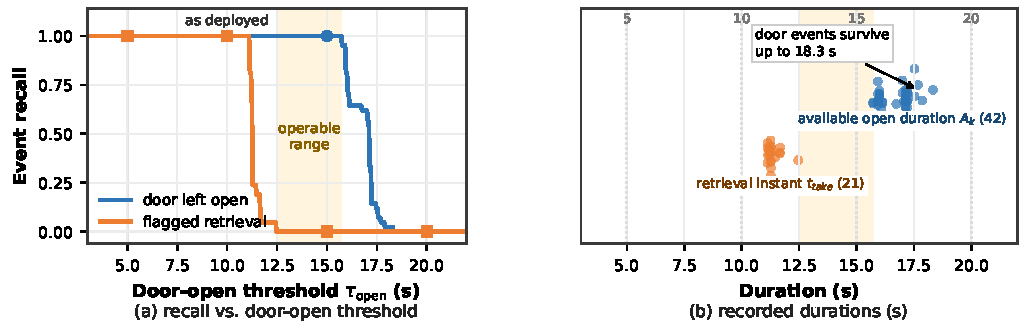
\includegraphics[width=0.98\textwidth]{figures/fig10_sensitivity.pdf}
\caption{Sensitivity to the door-open alarm threshold. Left: recall of the two
door-derived event types as a function of the threshold. Right: distribution of the
available open duration across the 42 door events, with the candidate thresholds marked;
the gap between the flagged-retrieval instants (11.1--12.5~s) and the door availability
(15.7--18.3~s) is a band (12.5--15.7~s) in which the door alarm still fires for every clip
but no retrieval-from-flagged event survives; full recall of both requires
$\tau_{\mathrm{open}}\le 11.1$~s.\label{fig:e10}}
\end{figure}

\subsection{Long-run behaviour on real, uncalibrated footage}
\label{sec:exp-cross}
Running the complete pipeline over all 15\,328 frames of the Avenue sequences probes the
behaviour on real imagery with no relation to the locker geometry (Figure~\ref{fig:e11}). With YOLOv8n the run
sustained 28.6~fps at a median inference cost of 33.0~ms, completed 535~s of continuous
processing, and never produced a frame without a detection (0 of 15\,328 frames; Wilson
95\% upper bound 0.03\%); the overall mean is 8.13 persons per frame. The more
instructive number is how \emph{often} events occurred: in 535~s of real footage the
uncalibrated geometry produced 19 alarm events---approximately one alarm every 28~s---all
of them from the door-derived classes, which is the direct consequence of a polygon that
does not correspond to a compartment sitting over arbitrary dark image content and
crossing the dark-ratio threshold intermittently. A deployment without calibration would
therefore be unusable, not because detection fails but because the geometric rules lose
their meaning. This is a design boundary, expressed in the currency an operator cares
about (alarms per minute), and it is why the system exposes no uncalibrated operating
mode. With HOG the same run produces a comparable event count through an entirely
different failure mode---18 events with essentially no persons detected---which shows that
the geometric channel and the person channel fail independently.

\begin{figure}[H]
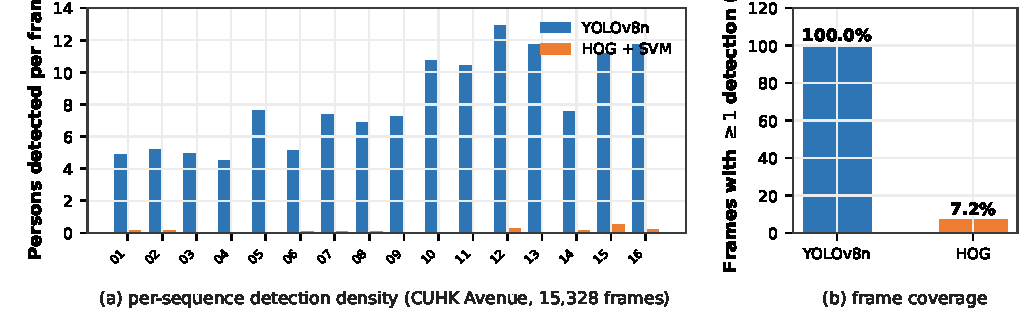
\includegraphics[width=0.98\textwidth]{figures/fig11_avenue.pdf}
\caption{Long-run behaviour on uncalibrated real footage (CUHK Avenue; (15\,328 frames, uncalibrated).
Left: persons detected per frame for each of the 16 sequences (YOLOv8n; HOG never exceeds
0.53 persons per frame). Right: share of frames containing at least one detection
(100\% versus 7.2\%).\label{fig:e11}}
\end{figure}
%%%%%%%%%%%%%%%%%%%%%%%%%%%%%%%%%%%%%%%%%%
\section{Field-Footage Study}
\label{sec:field}

The controlled experiments establish that the pipeline is correct under same-distribution
conditions and that its thresholds behave as declared. Neither question---does the system
work when the scene is not the one it was calibrated on, and what does it take to make an
unfamiliar site work---can be answered on rendered data by construction. This section
therefore reports the field study on the 15 recordings of Section~\ref{sec:field-corpus},
in three parts: the behaviour of the uncalibrated configuration (Section~\ref{sec:field-transfer}),
a validated door event on real footage (Section~\ref{sec:field-door}), and the two audits
that predict and repair the observed failures (Section~\ref{sec:audit}).

The field recordings carry no frame-level ground truth; results in this section are
therefore \emph{measured system behaviour}, supported by manual verification of specific
episodes and frames rather than precision/recall against labels. Every claim below is bounded to what the footage can
support, and the failure attributions were verified by inspecting the evidence snapshots
the system stores with every event.

\subsection{Uncalibrated transfer: what an unconfigured deployment does}
\label{sec:field-transfer}
The complete pipeline is run over each recording with the factory-default configuration
(i.e., the compartment grid and pickup polygon of the rendered benchmark, which correspond
to no real site). Over the corpus, the uncalibrated configuration emits 261 events in
1145~s---197 alarms and 64 informational events, i.e. one alarm every 5.8~s and one event
every 4.4~s (Table~\ref{tab:field}, last column;
Figure~\ref{fig:field12}, left). The distribution across recordings is itself informative.
The vendor demo with no people (v12) produces zero events, as it should. The static campus
bank (v04) produces 48, the two courier-deposit recordings (v01, v03) produce 20 and 74,
and the TV report (v11) produces 44. Three failure mechanisms account for the majority of
these alarms, and each was verified by inspecting the stored snapshots:

\begin{itemize}
\item \emph{Geometric mismatch.} The default compartment polygons land on arbitrary scene
content---in one snapshot they cover a person's torso, in another the centre of a real
locker bank with no relation to its actual doors (Figure~\ref{fig:field12}, right). Since
the dark-ratio statistic is meaningful only for a region that is actually a door, these
polygons cross the threshold intermittently; 77 of the 261 events are door-derived and
trace to this mechanism (10 door-left-open events in v03, 11 in v04, 7 in v11, and so on).
\item \emph{Colour collision.} The multiple-package rule misfires on warm-toned
apparel---in one snapshot the person's saturated yellow T-shirt is fragmented into
package-coloured blobs inside his own box, producing a spurious ``carrying 4 packages''
event. 146 of the 261 events are of this class.
\item \emph{Scenario mismatch.} Courier-deposit recordings legitimately contain people
carrying many packages; a rule-tuned for self-service retrieval misreads normal courier
work as an alarm even when the colour evidence is correct. This contributes to the same
146 and cannot be eliminated by recalibration---it is a vocabulary question, and it is
covered by the recommendation of Section~\ref{sec:discussion}.
\end{itemize}

These events should not be read as 261 individual false alarms; the meaningful statement
is that \emph{an uncalibrated deployment of this pipeline is unusable, and it is unusable
in three distinguishable, predictable ways.} The Avenue result (Section~\ref{sec:exp-cross}, one alarm per 28~s)
anticipated the first mechanism; the field corpus shows that on content dominated by
lockers and users the rate is more than six times worse, and it identifies the other two mechanisms,
which is exactly the material the audit of Section~\ref{sec:audit} turns into an
installation procedure.

\begin{figure}[H]
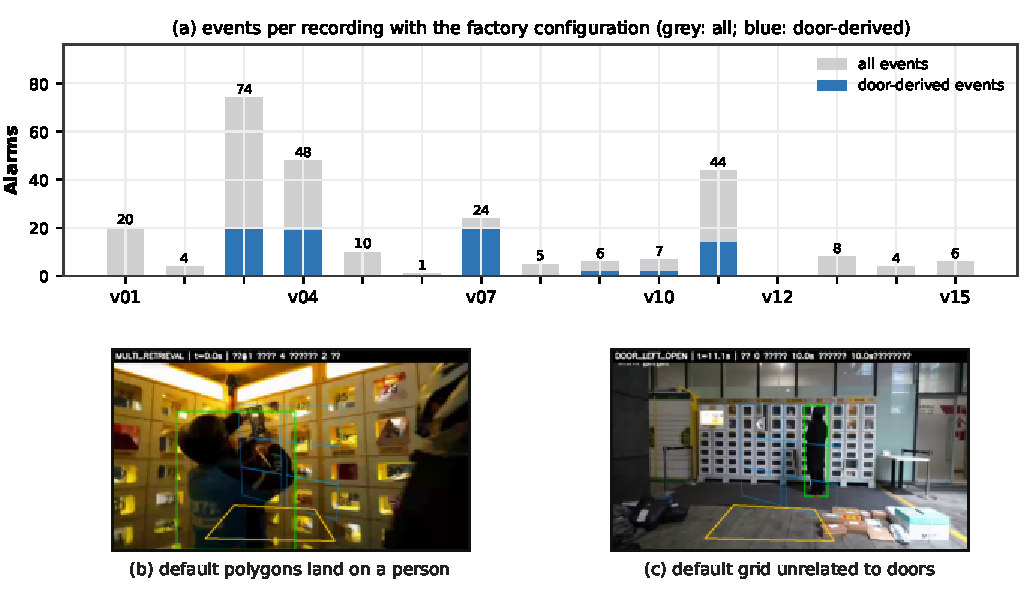
\includegraphics[width=0.98\textwidth]{figures/fig12_field_transfer.pdf}
\caption{Uncalibrated transfer on the field corpus. Left: events emitted per recording by the
factory-default configuration (grey: all events; darker bars: door-derived events),
against the recording duration on the secondary axis; v12 (no persons) is the control at
zero. Right: two evidence snapshots---the default polygons landing on a person's torso
(courier close-up) and on the centre of a real locker bank with no relation to its
doors.\label{fig:field12}}
\end{figure}

\subsection{A real door-left-open episode, measured by the system's own statistic}
\label{sec:field-door}
Among the recordings is a public-service clip whose subject is precisely the operational
problem this paper addresses: a Fengchao express-locker user retrieves a parcel and walks
away without closing the compartment. The episode is unambiguous and occupies a
camera-stable interval (median motion 0.2--1.3~px/frame between 6.2 and 24~s); the door
stands open for at least 5~s---the camera settles with the door already open, and a
subsequent user closes it at $\approx$11.3~s. It therefore provides a rare opportunity: a
real open door, on a real locker, in footage the system has never seen.

Four compartment-sized regions are defined by hand on this clip---the open compartment
($k^\ast$) and three neighbouring compartments used as controls---and the system's own
statistic \eqref{eq:dark}--\eqref{eq:door-decision} is evaluated over 6--21~s (sampled
every 0.2~s) with the deployed parameters ($\kappa=0.62$, $\eta=0.15$). The result
(Figure~\ref{fig:field13}) is a clean separation. While the door stands open
(6.3--9.2~s), the compartment reads $r_{k^\ast}=0.939$ on average with range
$[0.935,0.960]$ across the 13 unoccluded samples (standard deviation 0.007; 95\% CI of the
mean 0.934--0.943), while the three controls read 0.006, 0.011 and
0.030 (maxima 0.007, 0.013 and 0.031): every control sample stays below the 0.15
threshold, and the open compartment exceeds it by a factor of six. During the closing
interaction (9.4--13.0~s) the arriving user's body covers more than half of the
compartment in 18 of 19 samples (95\% CI 75.4--99.1\%); the estimator reports the state as
undecidable and
\emph{holds} it, exactly as the visibility policy prescribes, rather than sampling a
partially blocked region. After the correction---door closed, user gone
(13.5--21~s)---the same region reads 0.027 on average (range $0.000$--$0.040$), a factor
of roughly 35 below the open state and far under threshold, and the controls remain at or
below 0.11 throughout. The statistic therefore separates the three situations the state
machine must distinguish---open, closed, and undecidable---on real hardware, with the
deployed parameters and without any per-clip tuning.

Two readings matter here. First, the failure boundary established in
Section~\ref{sec:exp-cross} is a boundary of \emph{geometry}, not of the metric: given
regions that actually correspond to doors, the darkness-ratio statistic transfers to real
hardware (a real locker with dark viewing windows, under artificial light) without any
parameter change, with margins an order of magnitude wider than the threshold.
Second, the episode's duration (at least 5~s) is \emph{below} the deployed 10~s alarm
threshold, and the replay of Section~\ref{sec:exp-sens} already tells us what that means:
at $\tau_{\mathrm{open}}=5$~s this compartment would have been flagged promptly; at 10~s
it would not have alarmed at all had the arriving user been a little earlier. The field
episode therefore also calibrates intuition about $\tau_{\mathrm{open}}$ for real user
behaviour---open doors here last seconds, not the 15--18~s of our rendered clips---which is
part of why the threshold-audit replay is offered as a deployment tool rather than a
fixed recommendation.

\begin{figure}[H]
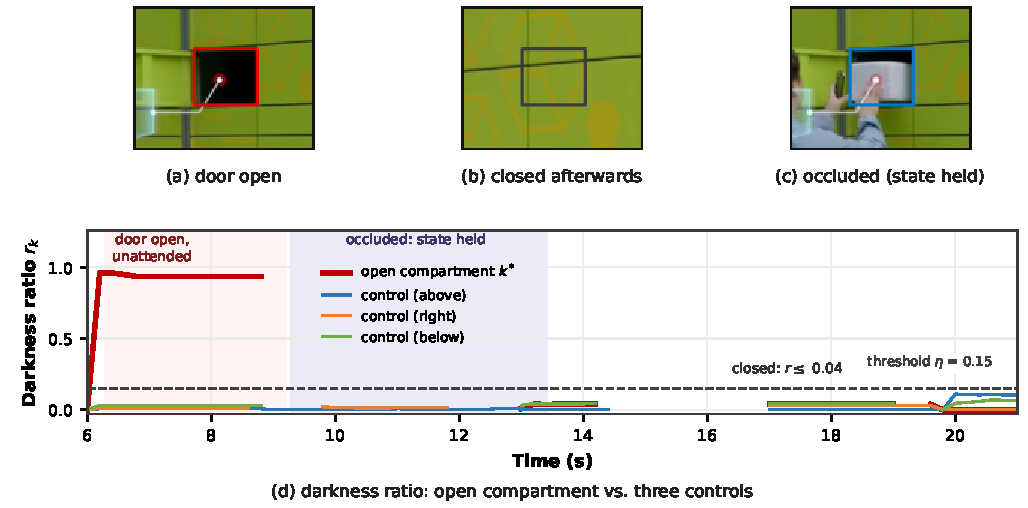
\includegraphics[width=0.98\textwidth]{figures/fig4_door.pdf}
\caption{The door statistic on a real open-door episode. Top: three frames of the episode
(door open; closed after the correction; the arriving user occluding the compartment),
with the calibrated region of the open compartment ($k^*$) outlined. Bottom: the darkness
ratio $r_k$ for the open compartment and three controls over 6--21~s; the red shading
marks the interval in which the door stands open, the blue shading the interval in which
the compartment is occluded by the arriving user and the state is held, and the dashed
line is the threshold $\eta=0.15$. The open compartment exceeds the threshold throughout;
every control sample stays below it.\label{fig:field13}}
\end{figure}

\subsection{Pre-deployment audits}
\label{sec:audit}
The field findings convert into two audits that run \emph{before} alarms are enabled, and
which we now define, measure on the corpus, and validate.

\subsubsection{Geometric audit}
The geometric audit is a coverage check during calibration: every compartment polygon is
overlaid on the reference frame, and the operator confirms (i) that each polygon contains
a door and fits it within a small tolerance, (ii) that the union of polygons covers the
locker front, and (iii) that the pickup polygon lies on the ground area in front of the
bank. The verification overlay is the same rendering used by the calibration tool
(Figure~\ref{fig:calib}, right). The failure it prevents is exactly the first mechanism of
Section~\ref{sec:field-transfer}: polygons that do not correspond to doors. Because the
check is visual and the calibration is one-time, its cost is minutes per site.

\subsubsection{Door-appearance audit and threshold recalibration}
The door statistic's second assumption---that a closed door is a bright, reflective
surface---does not hold universally. The static campus bank of the corpus (v04,
KaiPuxun-brand lockers) has doors with large smoked-glass viewing windows: the ``closed''
appearance already contains substantial dark area. Applying the audit to this site, we fit
twelve compartment cells on the static view, mask out person boxes as the system does, and
measure $r_k$ over 1152 samples across 240~s. The baseline distribution has median 0.292
and $p_{90}=0.328$---\emph{above} the default threshold $\eta=0.15$, which would classify
98.6\% of all samples as ``open'' (1136 of 1152; Wilson 95\% CI 97.8--99.1\%) on a locker
whose doors are overwhelmingly closed.
Recalibrating per site is straightforward because both modes are measurable: the audit
scans candidate thresholds and reports the fraction of samples classified ``open'', giving
0.5\% at $\eta=0.45$ and 0.3\% for $\eta\in[0.55,0.75]$ (Figure~\ref{fig:field14}, right).
Combined with the open-state reading of 0.94 measured on the episode of
Section~\ref{sec:field-door}, this places the safe range for this hardware at
$\eta'\in[0.45,0.75]$---below the open mode by at least $0.19$, above the closed $p_{90}$
by at least $0.12$. The audit output is therefore a per-site threshold recommendation with
measured margins, and it costs one pass over a sample of footage. This is the field
counterpart of the Chernoff argument \eqref{eq:chernoff}: on lockers with dark doors the
closed-state dark probability $\varepsilon_c$ must be measured, not assumed.

The recommendation was then closed in a loop, not merely illustrated. We re-ran the
complete pipeline on v04---the site the audit targets---in three configurations over its
full 240~s. With the factory-default geometry and threshold it emits 19 door-derived
events (6 \texttt{DOOR\_CLOSED}, 11 \texttt{DOOR\_LEFT\_OPEN}, 2
\texttt{FLAGGED\_DOOR\_RETRIEVAL}). Substituting the audited compartment geometry but
\emph{keeping} the default threshold $\eta=0.15$ leaves the misfire in place---20
door-derived events---because the recalibrated cells now measure the smoked-glass
appearance honestly and the unchanged threshold still calls it ``open''; this isolates
the threshold, rather than the geometry, as the operative defect at this site. Applying
the audit's recommended value with the same audited geometry ($\eta'=0.55$) removes
every door-derived event (19$\to$0). The audit is therefore not only diagnostic: its
output, applied as a configuration change, measurably repairs the failure it predicts,
and the events that remain on this site (43 in total) are the non-door, vocabulary-limited
classes discussed in Section~\ref{sec:discussion}, not door misfires.

\subsubsection{Colour-collision audit}
The colour-collision audit quantifies the risk behind the second failure mechanism before
it fires. For a sample of frames (here 1 frame per second), the audit runs person detection
and asks, for every person box, how many package-coloured blobs appear inside it; a frame
in which any person box contains at least two such blobs is a \emph{collision frame}---the
exact condition under which the multiple-package rule can misfire without any door or
geometry involvement. Over the corpus, 289 of 1020 person-frames (28.3\%; Wilson 95\% CI
25.7--31.2\%) are collision frames, with a per-site spread from 6.9\% (v04: 335
person-frames, 95\% CI 4.6--10.1\%) to 66.7\% (v14: six person-frames, 95\% CI 30--90\%); the
snapshot evidence
above shows the mechanism concretely. The audit does not automatically decide that a site
is bad: a collision frame may contain a person genuinely carrying warm-coloured packages
(as couriers do). What it provides is a triage: sites with a low collision rate (v04's
6.9\%, v06's 11.1\%) can enable the multiple-package rule as-is; sites above about a quarter
(Figure~\ref{fig:field14}, left; v01, v05, v10, v13 and v14 exceed 45\%) should either restrict the rule's domain
(courier-vs-user discrimination, or hand-region gating) or keep it in a report-only mode
until the colour model is adapted to the site. The audit runs in under a minute of video
per site and requires no calibration.

\begin{figure}[H]
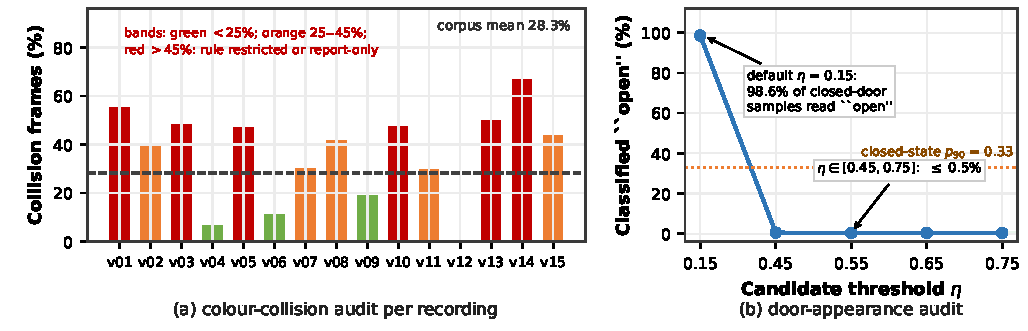
\includegraphics[width=0.98\textwidth]{figures/fig13_audits.pdf}
\caption{Pre-deployment audits. Left: colour-collision rate per recording (fraction of
person-frames whose person boxes contain at least two package-coloured blobs); the corpus
mean is 28.3\%. Right: door-appearance audit on the smoked-glass locker (v04): fraction of
samples classified ``open'' as a function of the candidate threshold $\eta$; the default
0.15 misclassifies 98.6\% of closed-door samples, while $\eta\in[0.45,0.75]$ leaves at most
0.5\%, with the open-state level (0.94, from the validated episode) far
above.\label{fig:field14}}
\end{figure}

\subsubsection{Detector sanity check on field footage}
As a final check that the perception front end survives the domain shift, person detection
was run on one frame per recording at 55\% duration. On every wide shot containing people
the detected boxes matched the visible persons (e.g., three persons at the static campus
site; single users at five further sites; two couriers at the deposit scenes), and no
detection was produced on person-free frames or title cards. Several recordings have no
person in the sampled frame (B-roll, screen close-ups), so this is reported as a
qualitative sanity check rather than a recall measurement; the numerical detector evidence
for the domain shift remains the COCO benchmark (Section~\ref{sec:exp-e2}) and the Avenue
run (Section~\ref{sec:exp-cross}), both of which the field check is consistent with.

%%%%%%%%%%%%%%%%%%%%%%%%%%%%%%%%%%%%%%%%%%
\section{Discussion}
\label{sec:discussion}

\subsection{What each class of evidence supports}
The experiments fall into four classes, and each supports a different kind of claim.

\emph{Correctness under same-distribution conditions} (Sections~\ref{sec:exp-e1}--\ref{sec:exp-cost}). The rendered benchmark is
produced by the same scene generator and uses the same calibrated geometry as the deployed
pipeline. The resulting scores verify that the implementation executes the specified
decision procedure, that the guards repair the failure modes they were designed for, and
that the declared thresholds behave as their definitions require---including the predicted
alarm latencies. They cannot estimate generalization to a locker we did not render, and no
such claim is made for the benchmark alone; the cross-scene set of
Section~\ref{sec:exp-variant}---re-rendered under a different camera and illumination with
the geometry re-calibrated for that view---is the deliberate exception, and it shows which
components carry over once the self-consistency is removed.

\emph{Parameter sensitivity} (Section~\ref{sec:exp-sens}). Replaying recorded timelines under alternative
thresholds shows how far the principal threshold can move before alarm behaviour changes,
and locates the two observable quantities that bound it. This is evidence about the method's
parameters: their usable range is measurable per site, at zero experimental cost.

\emph{Failure boundaries} (Sections~\ref{sec:exp-cross} and~\ref{sec:field}). On real footage with no calibration, the detector keeps
working and the geometric rules do not---one alarm per 28~s on Avenue, and one event per
4.4~s (197 alarms over 1145~s) on locker-dominated content---and the field evidence identifies
the three mechanisms behind
those numbers. This is the evidence that calibration is load-bearing rather than
convenient.

\emph{Transfer of the validated components} (Section~\ref{sec:field}). The door statistic's transfer is
established positively on a real episode with measured margins (0.94 versus 0.15, controls
$\le 0.11$ over the whole window and $\le 0.031$ while the door stood open), and its per-site
prerequisite ($\varepsilon_c$) is turned into a measured
audit. The colour-collision audit similarly converts a failure mechanism into a measurable
deployment-time quantity. What transfers are the \emph{metrics and their audits}; what must
be redone per site are the geometry and, on non-reflective doors, the threshold.

\subsection{When should a deployment choose rules, and when learning?}
The discussion in Section~\ref{sec:related} framed rule-based and learned anomaly detection
as ends of a trade-off rather than competitors. The measurements in this paper let that
trade-off be stated operationally. A rule-based pipeline is preferable when (i) the alarm
vocabulary is enumerable in advance---the operational concerns of a managed facility
usually are; (ii) alarms must be attributed and audited (which door, which quantity, which
threshold), because responsibility attribution at the facility is a first-class
requirement rather than a forensic afterthought; (iii) the compute budget excludes
server-side models; and (iv) the site geometry is stable, because the whole design turns
stability into calibration. Learned anomaly detection is preferable when the vocabulary
cannot be enumerated, when anomalies are defined by deviation from a data distribution
rather than by operational states, or when enough labelled or normal-only data exists to
train and the hardware budget permits. The two can coexist: the per-compartment
state-machine interface of this system is deliberately shaped so that a learned classifier
could replace any single predicate while keeping the audit chain---an obvious next step,
and one the ablation of Section~\ref{sec:exp-abl} would immediately police. What this paper adds to that
discussion is the cost side of the ledger: the calibration, the audits and the threshold
replays that make the rule-based side deployable are themselves measurable and cheap, and
they are what an operator must do anyway to explain to users what the system will and will
not detect.

\subsection{Positioning against existing rule-based and edge monitoring}
The contribution of this paper is easiest to state against the three bodies of work it is
closest to. Rule-based video-surveillance systems such as
iSurveillance~\cite{lim2014isurveillance} compose operator-defined spatial rules---tripwires,
region entry, dwell---and are, like this pipeline, interpretable by construction; their rules
are, however, specified by hand per camera and evaluated largely qualitatively, so neither the
usable range of a rule's parameters nor its site-to-site failure boundary is itself a measured
quantity. Locker- and retail-monitoring studies~\cite{ramoa2021door,santra2019retail} analyse
door and shelf interactions but report behaviour statistics rather than an actionable alarm
contract. Learned edge VAD (Section~\ref{sec:related}) scores deviation from a normality model
and can fit constrained hardware, but its output is a score, not an event attributed to a
compartment or a person. What is specific here is deliberately none of those: not a new
detector and not a new rule type, but the \emph{decomposition} of an enumerable alarm
vocabulary into calibrated geometric regions, named thresholds and per-compartment state
machines; the treatment of \emph{pre-deployment audits} as first-class measurements that
predict, before alarms are enabled, which rules will misfire at a given site; and the
\emph{replay} of recorded timelines to bound each threshold without re-runs. The field study
adds the measurement these approaches usually omit---how far the default configuration is from
usable on footage the system has never seen---and converts it into an installation procedure.
We do not claim a new anomaly-detection operator; we claim that the operator used is
calibrated, auditable and bounded, and that the bounds are measurable.

\subsection{Back to the large picture: supervision for unattended infrastructure}
The introduction framed the problem broadly: unattended delivery infrastructure is
becoming public infrastructure, and its supervision is currently reactive. The present
study is one instance, but the measured principles generalize to the class. First,
\emph{calibration-first} is a viable alternative to train-first for facilities with fixed
geometry: a one-time geometric calibration plus measured audits replaces the data appetite
of learned approaches, and the failure boundary it carries (Section~\ref{sec:exp-cross}) is
sharp, predictable, and testable at installation. Second, \emph{alarm auditability} is an
achievable and useful property, not a philosophical one: every event in this system names a
compartment, a quantity and a threshold, and the system stores the evidence snapshot; the
same discipline applies to any state-based anomaly vocabulary for lockers, vending
machines, or self-service kiosks. Third, \emph{audits before alarms} generalize: the
geometric and colour checks run here in minutes per site and prevent the dominant failure
modes at their root. Fourth, the limits generalize too: appearance-based proxies (colour,
darkness) are domain-dependent and must be measured per site; anything requiring
individual identification is out of scope for a privacy-preserving, appearance-only
system---and should remain so. For the operator of a multi-site network, the natural
rollout is therefore: calibrate, audit, run in report-only mode for a soak period, then
enable alarms after replaying thresholds on the site's own footage---a workflow this paper
supports tool-by-tool rather than as a slogan.

\subsection{Scaling, cost and privacy, closed}
The cost model \eqref{eq:costmodel} and the measurements of Section~\ref{sec:exp-cost} bound a single machine at
one 15--25~fps view comfortably, with the observation stage nearly free compared with
detection. Serving several lockers per machine requires either a geometric cascade---keeping
the cheap per-compartment estimator on every view and running deep detection only on views
whose door state changed---or one process per view sharing an event store; both are
compatible with the present interfaces and neither is implemented here, so the claim we
make is the measured envelope, not a plan. On privacy, the design is conservative by
construction: all processing is local, every event stores a snapshot, and no face
recognition or identity inference exists anywhere in the pipeline; the field corpus was
used strictly as input footage, with aggregate statistics and a handful of frames reported.
Any deployment should still be transparent to the facility's users about the existence and
purpose of the monitoring---the survey numbers of Section~\ref{sec:intro} suggest users
support supervision that is non-intrusive, which is an obligation as much as an
opportunity.

\subsection{Limitations}
Several limitations bound the claims above. The same-distribution scores of
Section~\ref{sec:exp-e1} verify the pipeline, not generalization; the cross-scene set of
Section~\ref{sec:exp-variant} removes that self-consistency, and shows the score falling to
an event-level $F_1$ of 0.857 with the colour-proxy rule the only component that fails. The field study, while
quantitative, is a study of 15 recordings rather than a deployment: the recordings carry no
frame-level ground truth, so no event-level precision or recall is reported for the
calibrated configuration on real sites; what is reported is measured system behaviour,
together with the audit loop of Section~\ref{sec:audit}, which is closed at the event-count
level on a single site (v04) and will need per-site repetition. Establishing calibrated
end-to-end precision and recall requires annotated field footage and a live installation. The
field recordings carry no anomaly annotations, so event-level precision and recall is not
computable on this corpus; we report measured system behaviour and individually verified
episodes instead of unverified rate estimates, and release the annotation and scoring tooling
for future annotated deployments. Every rate we do report carries a Wilson interval, and on the low-count
sites those intervals are deliberately wide---v14's 66.7\% rests on six person-frames
(95\% CI 30--90\%) and should be read as a direction rather than an estimate. Our
comparison against learned anomaly detection is analytic (Section~\ref{sec:discussion})
rather than experimental: no learned VAD checkpoint was trained or run head-to-head here,
so the claim that a rule pipeline is preferable under the stated constraints rests on the
attribution and auditability requirements, not on a measured accuracy advantage, and a
learned-per-predicate variant remains an untested upgrade path. All timings are
single-machine, single-run measurements on one CPU, with the load comparisons of
Section~\ref{sec:exp-cost} as the only sensitivity control.

The remaining limits are perceptual and lexical. The door statistic is a
binary proxy for a physical state and is bounded by its appearance definition; on lockers
with non-reflective doors it requires the measured recalibration demonstrated in
Section~\ref{sec:audit}, and on lockers whose doors are visually unlike either of our two
hardware examples, the audit must be run rather than assumed. The colour proxy for
packages is tuned for the warm-toned food containers and bags of the target domain and is
explicitly guarded by the collision audit; a deployment in a different packaging culture
should re-measure it. Finally, the courier-versus-user ambiguity noted in
Section~\ref{sec:field-transfer} is a vocabulary limitation of the current rule set, not a
perception failure, and resolving it (e.g., by shift-based courier modelling) is future
work.

%%%%%%%%%%%%%%%%%%%%%%%%%%%%%%%%%%%%%%%%%%
\section{Conclusions}
\label{sec:conclusions}
This paper developed and evaluated an auditable anomaly detection layer for unattended
delivery lockers under a CPU-only, open-source, fully local budget. The system estimates
the state of every compartment from calibrated image regions, tracks users with explicit
guards against measured detector failure modes, and raises six event types through
per-compartment rules whose every threshold is a named, documented parameter; each alarm
therefore names a compartment, a measured quantity and a threshold, and can be audited
after the fact. Correctness under same-distribution conditions is established on a
119-clip benchmark (perfect clip- and event-level scores, interpreted as implementation
verification rather than generalization), the mechanism contributions are isolated
by a paired ablation, and the door threshold's usable range is bounded by an analytic
replay that reproduces measured counts exactly and requires no re-runs. The field study
completes the picture on the other side of the boundary: uncalibrated deployment of this
pipeline is unusable (261 events over 1145~s of real locker footage, 197 of them alarms---
one event every 4.4~s---in three verified mechanisms), while a real door-left-open episode is
detected by the system's own statistic
with wide margins (0.94 versus a 0.15 threshold, controls below 0.04 during the episode), and the two
pre-deployment audits---geometric coverage, and door-appearance plus colour-collision
measurement---convert those findings into an installation-time procedure with measured
outputs. The transferable parts of the work are the calibration-to-rules decomposition, the
audit-before-alarms discipline, and the parameter replay; the parts that must be redone
per site are exactly the parts the audits measure.

For an operator the practical reading is narrow and deliberate: run the audit, calibrate,
soak in report-only mode, replay the thresholds against the site's own footage, and only
then let the system alarm---and expect each alarm it does raise to be checkable against a
stored snapshot and a named threshold. For a researcher, the open frontier this study
leaves is the courier-versus-user vocabulary and the learned-per-predicate upgrade path,
both of which the present interface was designed to accommodate.

%%%%%%%%%%%%%%%%%%%%%%%%%%%%%%%%%%%%%%%%%%
% 文末声明区（MDPI 顺序：Author Contributions → Funding → IRB → Informed Consent →
% Data Availability → Acknowledgments → Conflicts of Interest → Abbreviations）
% 注意：mdpi.cls 没有 \backmatter 命令，声明命令直接紧随正文之后。
%%%%%%%%%%%%%%%%%%%%%%%%%%%%%%%%%%%%%%%%%%

\authorcontributions{The author is the sole contributor to this work: conceptualization,
methodology, software, validation, formal analysis, investigation, resources, data
curation, writing---original draft preparation, writing---review and editing,
visualization, supervision, project administration, and funding acquisition. The author
has read and agreed to the published version of the manuscript.}

\funding{This work was supported by the Undergraduate Innovation and Entrepreneurship
Training Program of Northeast Forestry University (project number to be assigned upon
provincial-level approval).}

\institutionalreview{Not applicable. This study did not involve humans or animals; all
analyzed video material consists of publicly available recordings and programmatically
generated synthetic data.}

\informedconsent{Not applicable.}

\dataavailability{The rendered behaviour benchmark is produced programmatically by the
scene-generation scripts of the project and can be regenerated from the released code; the
COCO val2017 dataset and the CUHK Avenue dataset are publicly available from their
original distributors. The field recordings analyzed in Section~\ref{sec:field} are
publicly available videos published on video-sharing platforms; the evaluation logs record
each recording's published title, and the recordings are used as inputs for analysis only
and are not redistributed. The complete system---source code, configuration files, the geometric and
door-appearance calibration tools, the pre-deployment audit tools, the experiment
drivers and the evaluation scripts---together with the evaluation logs
(\texttt{logs/*.json}) from which the numbers in this paper are derived, is openly
available at \url{https://github.com/LuoluoKing/locker-audit-vision}. The scripts
that regenerate the field-study measurements are
\texttt{tools/analyze\_field\_videos.py} (corpus survey),
\texttt{tools/eval\_field.py} (per-recording event timelines),
\texttt{tools/field\_color\_audit.py} (colour-collision audit),
\texttt{tools/field\_door\_probe.py} and \texttt{tools/field\_study.py} (door-state
and compartment dark-ratio time series), and
\texttt{tools/analytic\_threshold\_sensitivity.py} (threshold replay).}

\acknowledgments{The author thanks the campus users who participated in the questionnaire
reported in Section~\ref{sec:setup}. During the preparation of this manuscript, the author
used an AI-based assistant (WorkBuddy, based on a large language model) for LaTeX
typesetting assistance, code generation for the evaluation scripts, and language editing;
the author has reviewed and edited all outputs and takes full responsibility for the
content of this publication.}

\conflictsofinterest{The author declares no conflicts of interest.}

\abbreviations{Abbreviations}{%
The following abbreviations are used in this manuscript:

\noindent
CPU: Central processing unit\\
COCO: Common Objects in Context (dataset)\\
HOG: Histogram of oriented gradients\\
HSV: Hue, saturation, value (colour space)\\
IoU: Intersection over union\\
AP: Average precision\\
SVM: Support vector machine\\
VAD: Video anomaly detection
}

%%%%%%%%%%%%%%%%%%%%%%%%%%%%%%%%%%%%%%%%%%
\reftitle{References}

\bibliography{refs}

\end{document}
